% !TeX program = xelatex
% FPGA course design comprehensive report

\documentclass[12pt,a4paper]{ctexart}
\usepackage{GDUTReport}
\usepackage{float}
\usepackage{enumitem}
\usepackage{multirow}
\usepackage{makecell}
\usepackage{tabularx}
\usepackage{pdfpages}

\usetikzlibrary{positioning}
\graphicspath{{figures/}}
\setlength{\headheight}{20pt}
\setstretch{1.45}
\setmainfont{Times New Roman}
\hypersetup{
    colorlinks=true,
    linkcolor=black,
    citecolor=black,
    urlcolor=integratedblue
}
\setlist[itemize]{leftmargin=2em,itemsep=0.2em,topsep=0.2em}
\setlist[enumerate]{leftmargin=2em,itemsep=0.2em,topsep=0.2em}

\newcommand{\figtwocol}[6]{
    \begin{figure}[H]
        \centering
        \subfigure[#2]{\includegraphics[width=0.47\textwidth]{#1}}
        \hfill
        \subfigure[#4]{\includegraphics[width=0.47\textwidth]{#3}}
        \caption{#5}
        \label{#6}
    \end{figure}
}

\newcommand{\figone}[4]{
    \begin{figure}[H]
        \centering
        \includegraphics[width=#1\textwidth]{#2}
        \caption{#3}
        \label{#4}
    \end{figure}
}

{
    \title{FPGA课程设计报告}
    \subtitle{基于ZYNQ7020的图像采集、边缘检测与HDMI显示系统}
    \name{黎嘉亮}
    \thenumber{3123009617}
    \major{微电子科学与工程}
    \class{2班}
    \team{菲菲公组}
    \teacher{周贤中}
}

\begin{document}

\pagenumbering{gobble}
\makecover

\newpage
\begin{abstract}
本课程设计围绕 ZYNQ7020 图像处理实验展开，从纯 RTL 仿真开始，逐步完成 HDMI 图案显示、Sobel 边缘检测、UART 图像传输、PS/PL 联合显示控制，以及第二周综合拓展。整个系统以 Verilog 图像流水线为核心，配合 PS 端 C 程序和 PC 端 Python 上位机，实现了从图片或摄像头输入、串口发送、BRAM 缓存、灰度与边缘计算，到 HDMI 输出显示的完整链路。

本组在基础实验中完成了 \verb|sobel_00| 至 \verb|sobel_05| 的仿真、上板和现象记录；在小扩展中分别加入了红色边框显示、Sobel 反色显示、UART 图像边框标识等功能；在综合拓展中重点改造上位机输入规格，使其支持目标尺寸选择、缩放策略选择以及新增图片输入规格，并保持原图、灰度、边缘、叠加与阈值控制等显示命令可用。报告按照实验推进顺序记录设计思路、关键修改、验证现象、资源占用和调试问题。

\par
\textbf{关键词：} ZYNQ7020；FPGA；Sobel 边缘检测；UART；HDMI；BRAM；上位机
\end{abstract}

\tableofcontents
\clearpage
\pagenumbering{arabic}
\setcounter{page}{1}

\section{课程设计总体说明}

\subsection{项目目标}

本次课程设计的主线是把图像处理链路拆成几个可以逐步验证的小实验。前半部分先用 RTL 仿真确认 Sobel 处理核心的正确性，再在开发板上验证 HDMI 时序和图像输出；中间部分加入 UART 和 PS 端程序，使 PC 端图像能够通过串口写入 BRAM；最后在 \verb|sobel_05_pc_control_display| 的基础上实现显示模式控制和输入规格扩展。

从实现角度看，本项目不是单一模块开发，而是一次从算法、时序、接口到上板调试的完整组合。我们最终需要回答三个问题：第一，图像数据能不能稳定进入 FPGA；第二，PL 侧流水线能不能正确完成灰度和 Sobel 处理；第三，HDMI 输出、显示控制和上位机交互能不能在真实板卡上跑通。

\subsection{实验环境}

\begin{table}[H]
\centering
\caption{实验软硬件环境}
\begin{tabular}{p{0.28\textwidth}p{0.60\textwidth}}
\toprule
项目 & 内容 \\
\midrule
开发板 & ZYNQ7020 开发板，器件型号 \verb|xc7z020clg400-2| \\
开发工具 & Vivado 2017.4，Xilinx SDK，ModelSim/Icarus Verilog，Python \\
图像接口 & HDMI 显示输出，USB-UART 串口传输 \\
主要语言 & Verilog HDL，C，Python \\
基础图像规格 & \verb|128 x 72|，RGB888 \\
综合拓展方向 & 基于 \verb|sobel_05| 的上位机与输入规格扩展 \\
\bottomrule
\end{tabular}
\end{table}

\subsection{总体数据流}

几个实验的功能逐步叠加，但核心数据路径保持一致。PC 端先把图像转换为约定尺寸和 RGB888 字节流，通过 UART 发给 PS；PS 端按帧头、行头和像素数据解析后写入 BRAM；PL 端从 BRAM 读取像素，完成灰度、Sobel 和显示模式选择，最终通过 HDMI 显示。

\begin{center}
\begin{tikzpicture}[
    node distance=1.35cm,
    block/.style={draw, rounded corners, align=center, minimum width=2.3cm, minimum height=0.85cm, fill=gray!8},
    arrow/.style={->, thick}
]
\node[block] (pc) {PC 上位机\\图片/摄像头};
\node[block, right=of pc] (uart) {UART\\帧协议};
\node[block, right=of uart] (ps) {PS 端 C 程序\\帧解析};
\node[block, right=of ps] (bram) {AXI BRAM\\图像缓存};
\node[block, below=of bram] (pl) {PL 图像流水线\\灰度/Sobel/控制};
\node[block, left=of pl] (hdmi) {HDMI 输出\\显示器};
\draw[arrow] (pc) -- (uart);
\draw[arrow] (uart) -- (ps);
\draw[arrow] (ps) -- (bram);
\draw[arrow] (bram) -- (pl);
\draw[arrow] (pl) -- (hdmi);
\end{tikzpicture}
\end{center}

\subsection{小组分工}

小组分工按实验内容和联调环节拆分。实际推进时并不是完全割裂的，比如上位机和 PS 端会反复联调，PL 显示控制和时序验证也需要一起看；表中的分工主要对应每个人负责推进和整理的主任务。

\begin{longtable}{@{}C{0.10\textwidth}C{0.16\textwidth}p{0.50\textwidth}C{0.08\textwidth}@{}}
\caption{小组分工表}\\
\toprule
成员 & 主要职责 & 具体工作内容 & 占比 \\
\midrule
\endfirsthead
\toprule
成员 & 主要职责 & 具体工作内容 & 占比 \\
\midrule
\endhead
黄煜盛 & 扩展实验开发、PL端联调 & 负责扩展实验 02、03、05 的代码编写与调试；综合拓展任务中 PL 端代码修改，包括 \verb|hdmi_bram_sobel_display.v|、\verb|sobel_core.v| 的尺寸参数适配思路和图像配置解析；参与 PL 与 PS 联调验证；整理实验报告材料。 & 25\% \\
\midrule
黎嘉亮 & 扩展实验开发、PS端开发 & 负责扩展实验 00、01、04 的代码编写与调试；综合拓展任务中 PS 端程序修改和地址规划，包括 \verb|main.c|、控制字地址迁移、BRAM 地址布局；整理仿真报告和综合报告。 & 25\% \\
\midrule
肖任科 & 上位机开发、PPT制作 & 负责综合拓展任务中上位机代码修改，包括 \verb|camera_uart_sender.py| 的缩放函数、\verb|camera_uart_gui.py| 的尺寸预设界面与缩放策略选择；整理演示 PPT 和汇报材料。 & 25\% \\
\midrule
陈智恒 & 仿真验证、视频制作、时序分析 & 负责显示控制行为模型与自动化验证用例编写；整理综合拓展 Vivado 时序分析，包括 Setup、Hold、Pulse Width；统计资源占用；完成演示视频剪辑与后期制作。 & 25\% \\
\bottomrule
\end{longtable}

\section{实验0：Sobel RTL 仿真}

\subsection{实验目标与数据格式}

实验 0 是后续上板实验的预验证。该实验不依赖 HDMI 或开发板，直接用 testbench 生成 UART 字节流，驱动 \verb|uart_rx|、\verb|image_frame_rx|、\verb|rgb_to_gray|、\verb|sobel_core| 和视频输出模型，最后把处理结果导出为图像文件。

仿真使用的图像格式为 \verb|128 x 72|、RGB888。UART 图像帧采用小端宽高字段，帧头和行头如下：

\begin{lstlisting}[language={},caption={UART 图像帧格式}]
frame header: 55 AA width_l width_h height_l height_h 18
line header : 33 CC row_l row_h
pixel data  : R G B, repeated 128 times per row
\end{lstlisting}

其中 \verb|18| 表示 RGB888 格式。testbench 除了正常图像外，也构造了错误帧头、错误格式和错误行号等情况，用来确认接收状态机不会把异常数据继续送入 Sobel 处理链路。

\subsection{关键模块}

\begin{itemize}
    \item \verb|uart_rx|：按照设定波特率恢复串口数据，输出 8 位并行字节和有效脉冲。
    \item \verb|image_frame_rx|：识别帧头、行头、行号和 RGB 像素，输出像素坐标及 RGB 数据。
    \item \verb|rgb_to_gray|：将 RGB888 转换为灰度数据，为 Sobel 核心准备输入。
    \item \verb|sobel_core|：维护 3 行窗口，计算横向与纵向梯度，并输出边缘强度。
    \item \verb|video_stream_model|：模拟一帧视频输出，生成 \verb|sobel_out.pgm| 和波形结束信号。
\end{itemize}

\subsection{仿真结果}

\figtwocol{exp0_input.png}{默认输入图像}{exp0_sobel.png}{默认 Sobel 输出}{实验0默认图像仿真结果}{fig:exp0-default}

默认图像包含矩形边框和对角线，边缘比较清楚，适合观察 Sobel 输出是否只在亮暗变化处产生响应。图 \ref{fig:exp0-default} 中可以看到，输出结果保留了输入图像的主要边缘，说明灰度转换和 Sobel 计算链路能够正常工作。

\figtwocol{exp0_alt_input.png}{扩展输入图像}{exp0_alt_sobel.png}{扩展输入 Sobel 输出}{实验0更换输入图像后的结果}{fig:exp0-alt}

更换输入图案后，Sobel 输出随图像结构变化，边缘响应集中在亮度突变的位置。这一部分主要用于确认处理链路不是只对默认样例有效。

\subsection{关键波形}

\figone{0.96}{exp0_wave_full.png}{实验0完整仿真波形}{fig:exp0-wave-full}

完整波形用于确认一帧图像从 UART 输入到视频输出的全流程，重点观察帧开始、像素有效、灰度有效、边缘有效和帧结束信号之间的时序关系。

\figone{0.82}{exp0_wave_local.png}{实验0局部有效信号波形}{fig:exp0-wave-local}

局部波形放大后可以更直观看到流水线延迟：\verb|rgb_valid| 先拉高，随后 \verb|gray_valid|、\verb|edge_valid| 和 \verb|video_valid| 依次出现。该现象符合图像处理流水线逐级寄存的特点，也说明各模块之间的 valid 信号没有乱序。

\section{实验1：HDMI 固定图案显示}

\subsection{基础功能}

实验 1 的重点是先把 HDMI 时序跑通。PL 端根据像素坐标生成固定测试图案，输出到 HDMI 显示器。这个实验虽然没有 Sobel 算法，但它验证了像素时钟、行场同步、坐标计数和 RGB 输出，是后续所有显示实验的基础。

\figtwocol{exp1_basic.jpg}{基础图案显示}{exp1_extend.jpg}{红色边框扩展}{实验1基础与扩展现象}{fig:exp1-phenomenon}

\subsection{扩展实现}

扩展功能是在原 HDMI 图案上加入红色边框。实现时在 \verb|hdmi_image_display.v| 中根据当前像素坐标判断是否位于边框区域：若位于边框，则输出红色；否则保持原图案显示。该修改只影响 RGB 选择逻辑，不改变 HDMI 时序和分辨率参数。

\begin{lstlisting}[style=Verilog,caption={实验1红色边框逻辑示意}]
wire border_on;
assign border_on = (x >= BORDER_X0 && x < BORDER_X1 &&
                    y >= BORDER_Y0 && y < BORDER_Y1) &&
                   (x < BORDER_X0 + BORDER_W ||
                    x >= BORDER_X1 - BORDER_W ||
                    y < BORDER_Y0 + BORDER_W ||
                    y >= BORDER_Y1 - BORDER_W);

assign rgb_out = border_on ? 24'hFF0000 : pattern_rgb;
\end{lstlisting}

\subsection{资源与时序}

\figtwocol{exp1_utilization.png}{资源占用}{exp1_timing.png}{时序结果}{实验1综合实现结果}{fig:exp1-timing}

从资源占用看，边框判断只增加少量比较和组合选择逻辑；从时序看，工程能够完成综合和实现，说明该扩展没有破坏原有 HDMI 显示链路。

\section{实验2：HDMI Sobel 边缘检测}

\subsection{基础功能}

实验 2 在 HDMI 图像显示的基础上加入 Sobel 边缘检测。图像数据在 PL 端经过灰度转换和 Sobel 核心后，显示边缘检测结果。该实验的重点是把实验 0 已经验证过的图像处理模块接入真实 HDMI 显示链路。

\figtwocol{exp2_basic.jpg}{基础 Sobel 显示}{exp2_extend.jpg}{反色边缘显示}{实验2基础与扩展现象}{fig:exp2-phenomenon}

\subsection{扩展实现}

扩展功能为 Sobel 结果反色显示。原本边缘强度越高，显示越亮；反色后重新计算显示灰度，使背景与边缘明暗关系反过来。这个修改位于显示输出阶段，不改变 Sobel 计算本身。

\begin{lstlisting}[style=Verilog,caption={实验2边缘反色逻辑示意}]
wire [7:0] edge_inv;
assign edge_inv = 8'hFF - edge_pixel;

assign rgb_out = {edge_inv, edge_inv, edge_inv};
\end{lstlisting}

\subsection{资源与时序}

\figtwocol{exp2_utilization.png}{资源占用}{exp2_timing.png}{时序结果}{实验2综合实现结果}{fig:exp2-timing}

反色显示只增加一个减法和输出选择，资源变化很小。上板现象中，边缘区域和背景区域的亮暗关系与基础版本相反，说明修改生效。

\section{实验3：UART 图像输入与 HDMI 显示}

\subsection{基础功能}

实验 3 开始引入 PS 端和 UART。PC 端上位机将图片或摄像头画面转成 \verb|128 x 72| RGB888 字节流，通过串口发送；PS 端接收并写入 BRAM；PL 端从 BRAM 读取像素，经 HDMI 放大显示。

\begin{figure}[H]
\centering
\subfigure[图像传输显示]{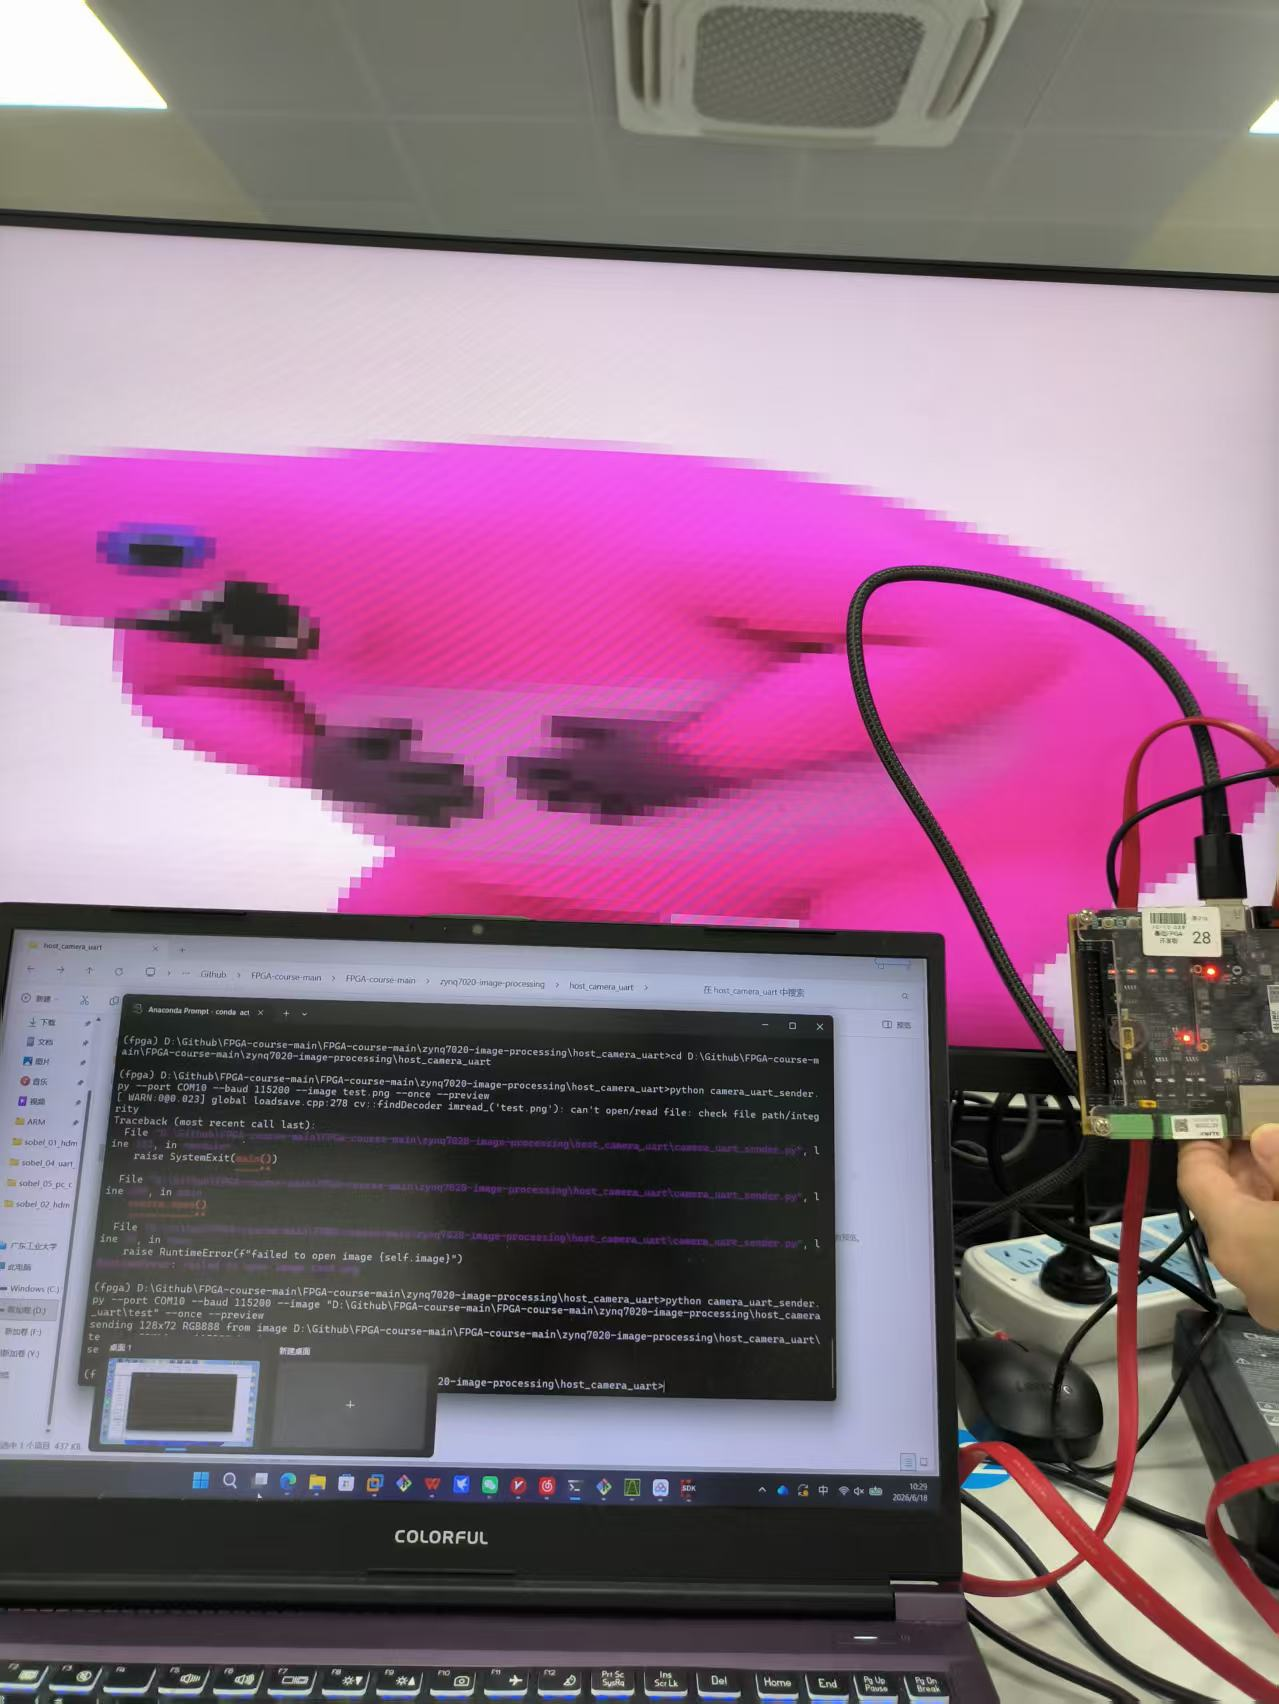
\includegraphics[width=0.31\textwidth]{exp3_basic1.jpg}}
\subfigure[串口信息记录]{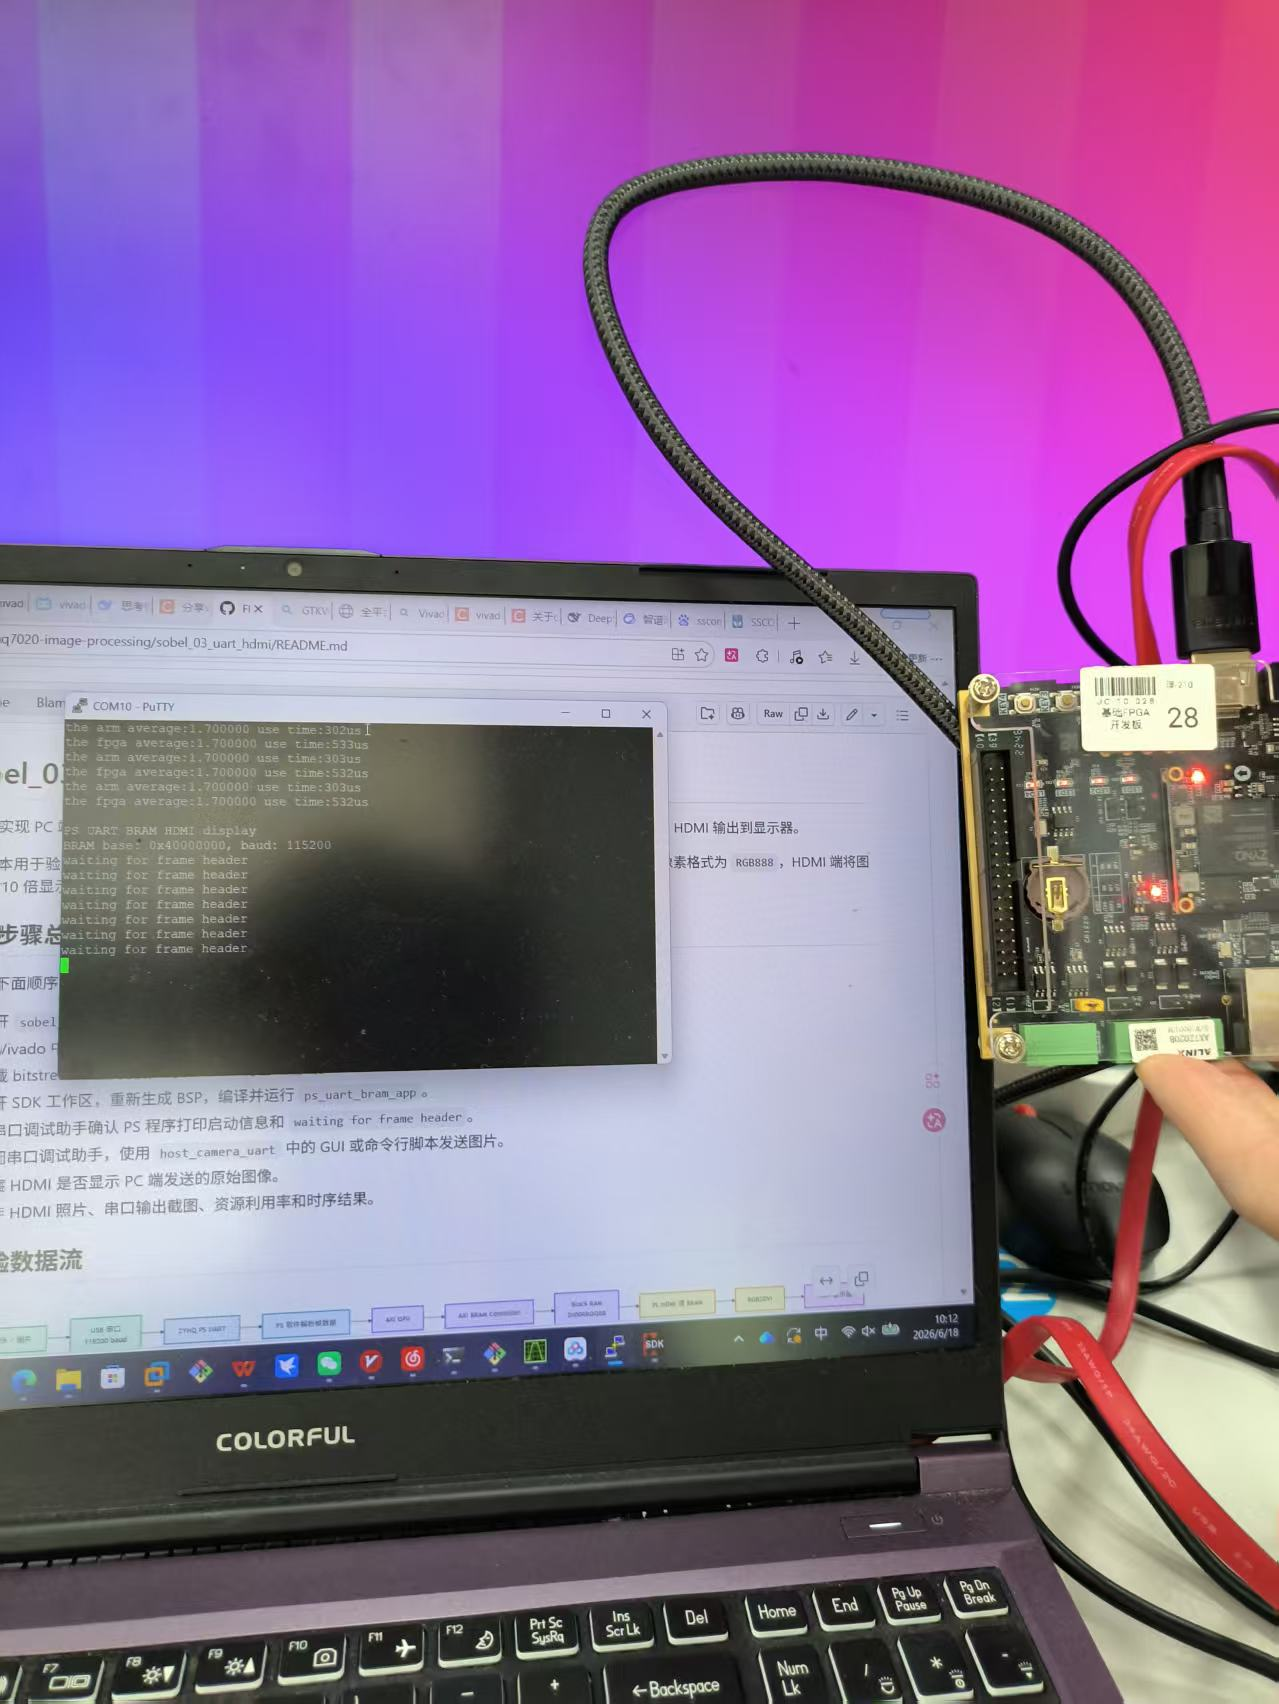
\includegraphics[width=0.31\textwidth]{exp3_basic2.jpg}}
\subfigure[摄像头输入显示]{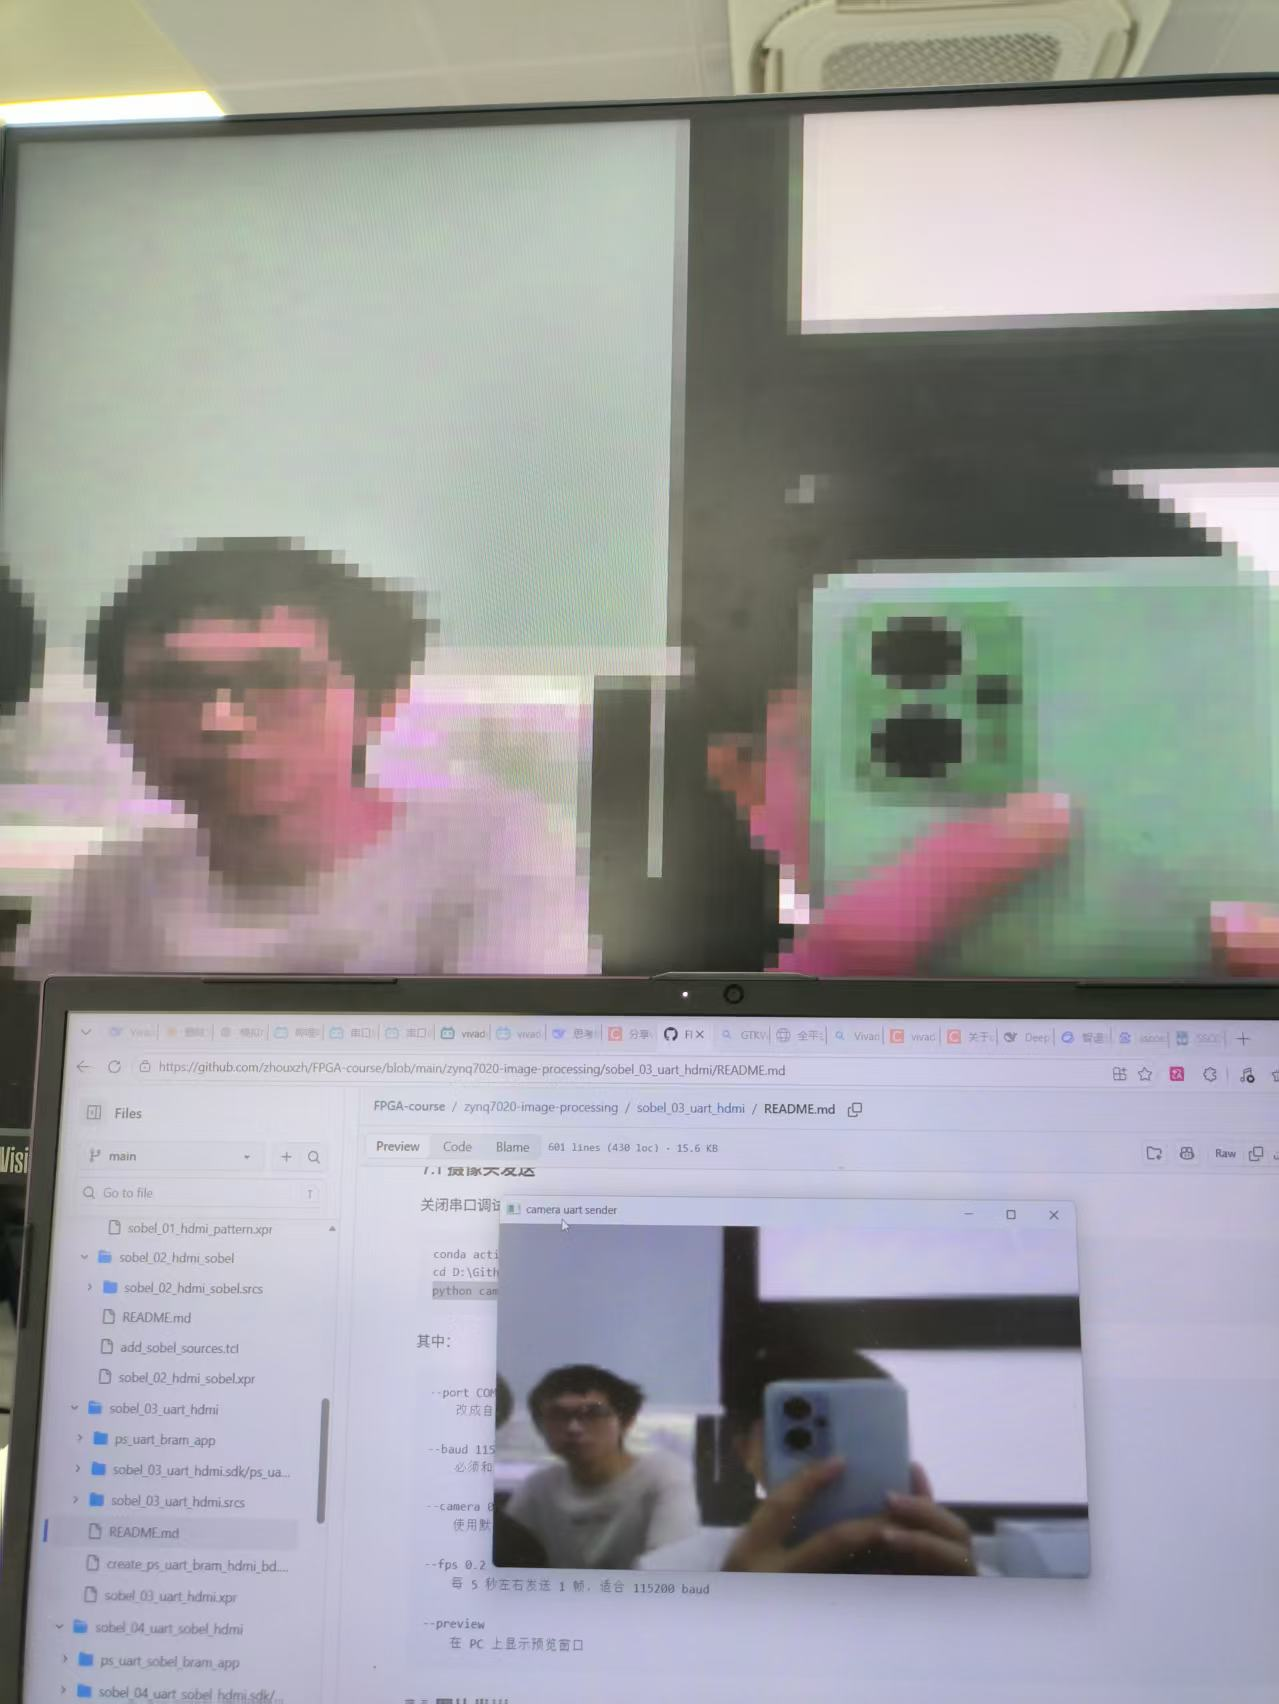
\includegraphics[width=0.31\textwidth]{exp3_basic3.jpg}}
\caption{实验3基础功能现象}
\label{fig:exp3-basic}
\end{figure}

从串口记录可以看到 PS 端处于等待帧头、接收帧、写 BRAM 的流程；从 HDMI 显示可以看到 PC 端输入图像已经显示到屏幕上。这个实验验证了 UART 帧协议和 BRAM 图像缓存链路。

\subsection{扩展实现}

实验 3 的扩展是在显示图像周围增加红色边框，并通过坐标偏移把低分辨率输入图像放置在 HDMI 输出区域的指定位置。主要修改在 \verb|hdmi_bram_display.v|：根据显示坐标计算映射后的图像坐标，判断是否位于图像区域或边框区域，再选择输出原图像、红色边框或背景。

\figone{0.62}{exp3_extend.jpg}{实验3红色边框扩展显示}{fig:exp3-extend}

\subsection{资源、时序与串口验证}

\begin{figure}[H]
\centering
\subfigure[资源占用]{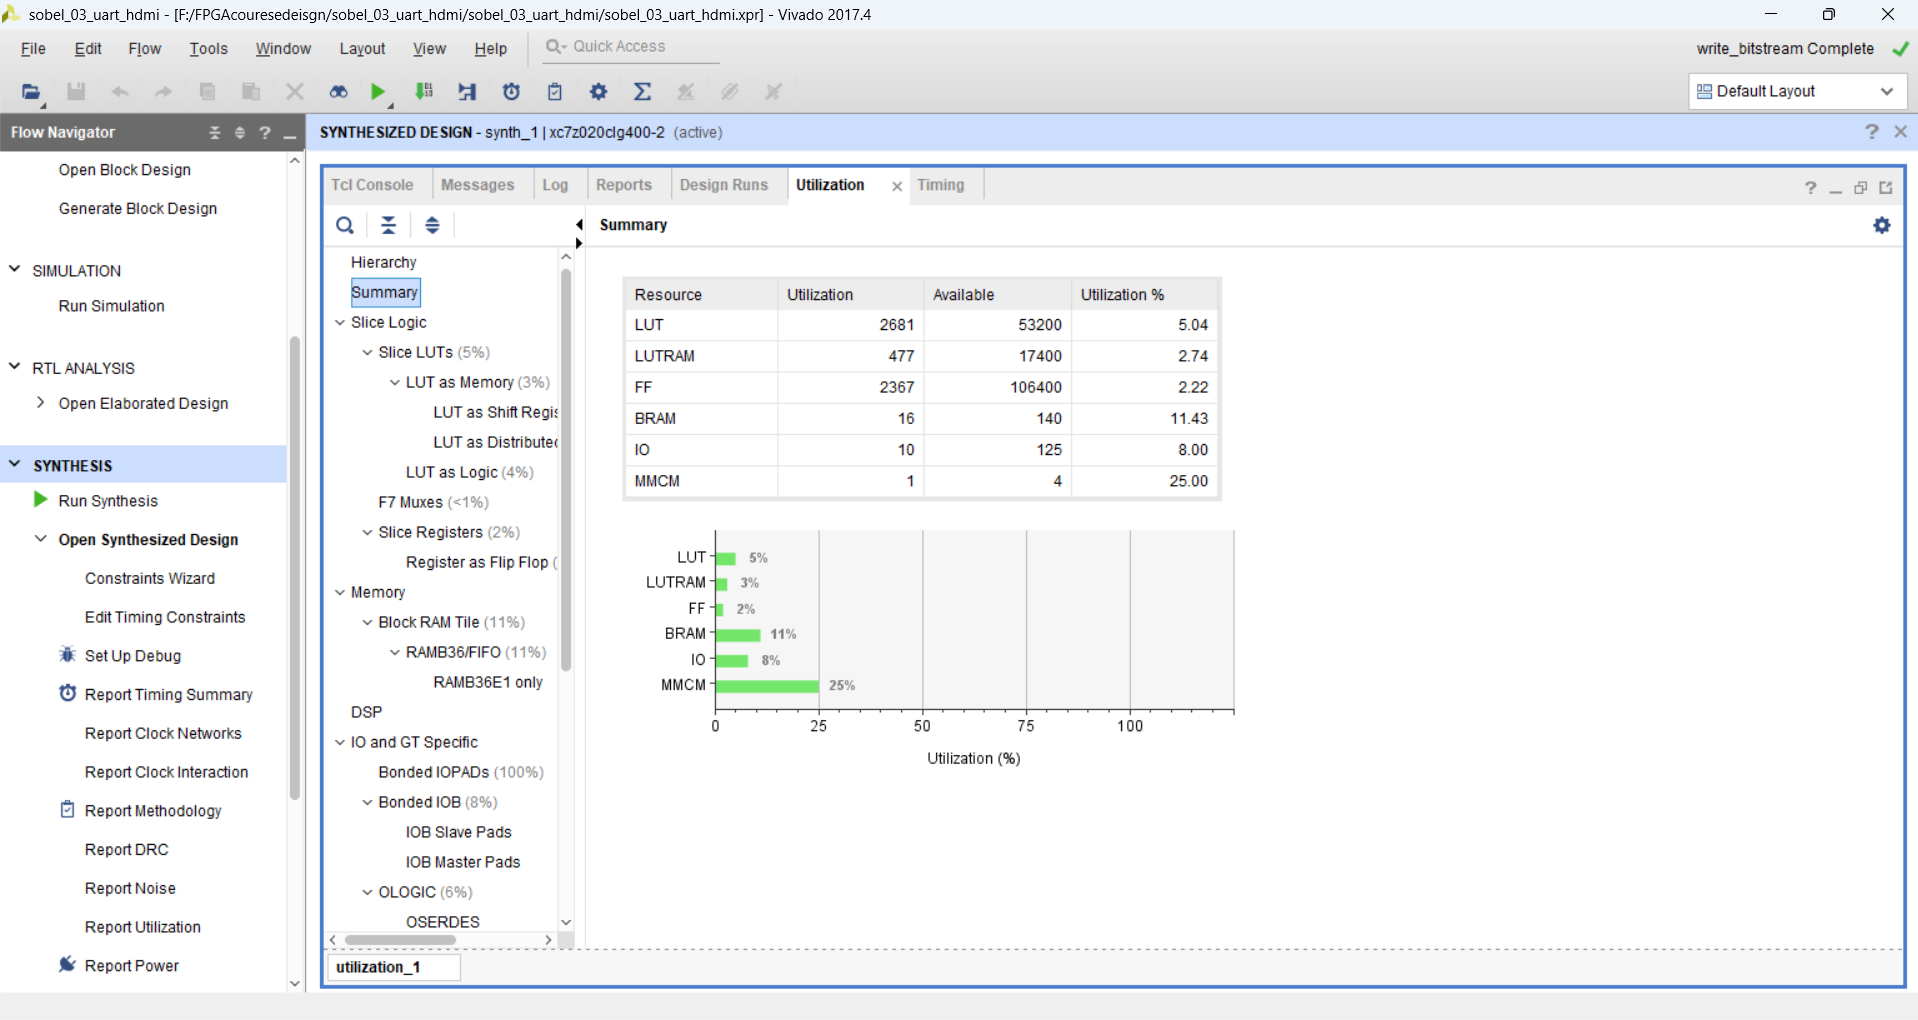
\includegraphics[width=0.32\textwidth]{exp3_utilization.png}}
\subfigure[时序结果]{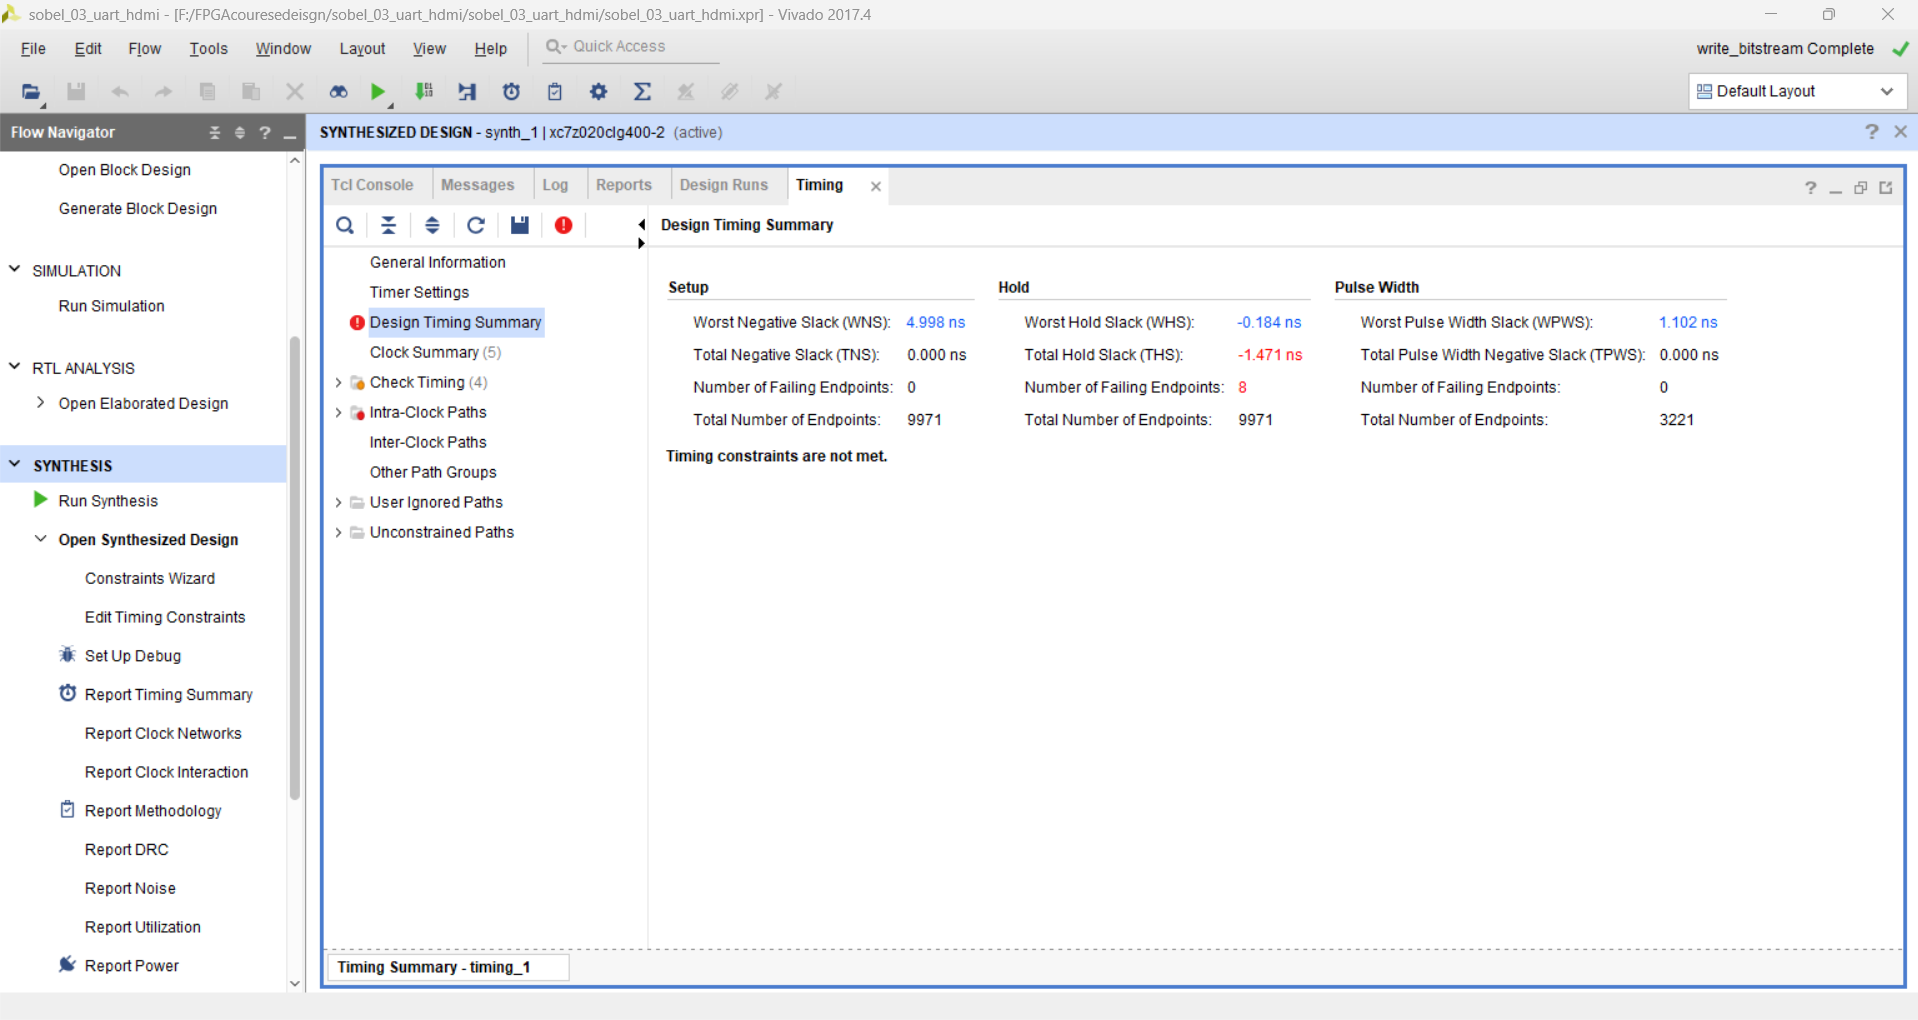
\includegraphics[width=0.32\textwidth]{exp3_timing.png}}
\subfigure[串口信息]{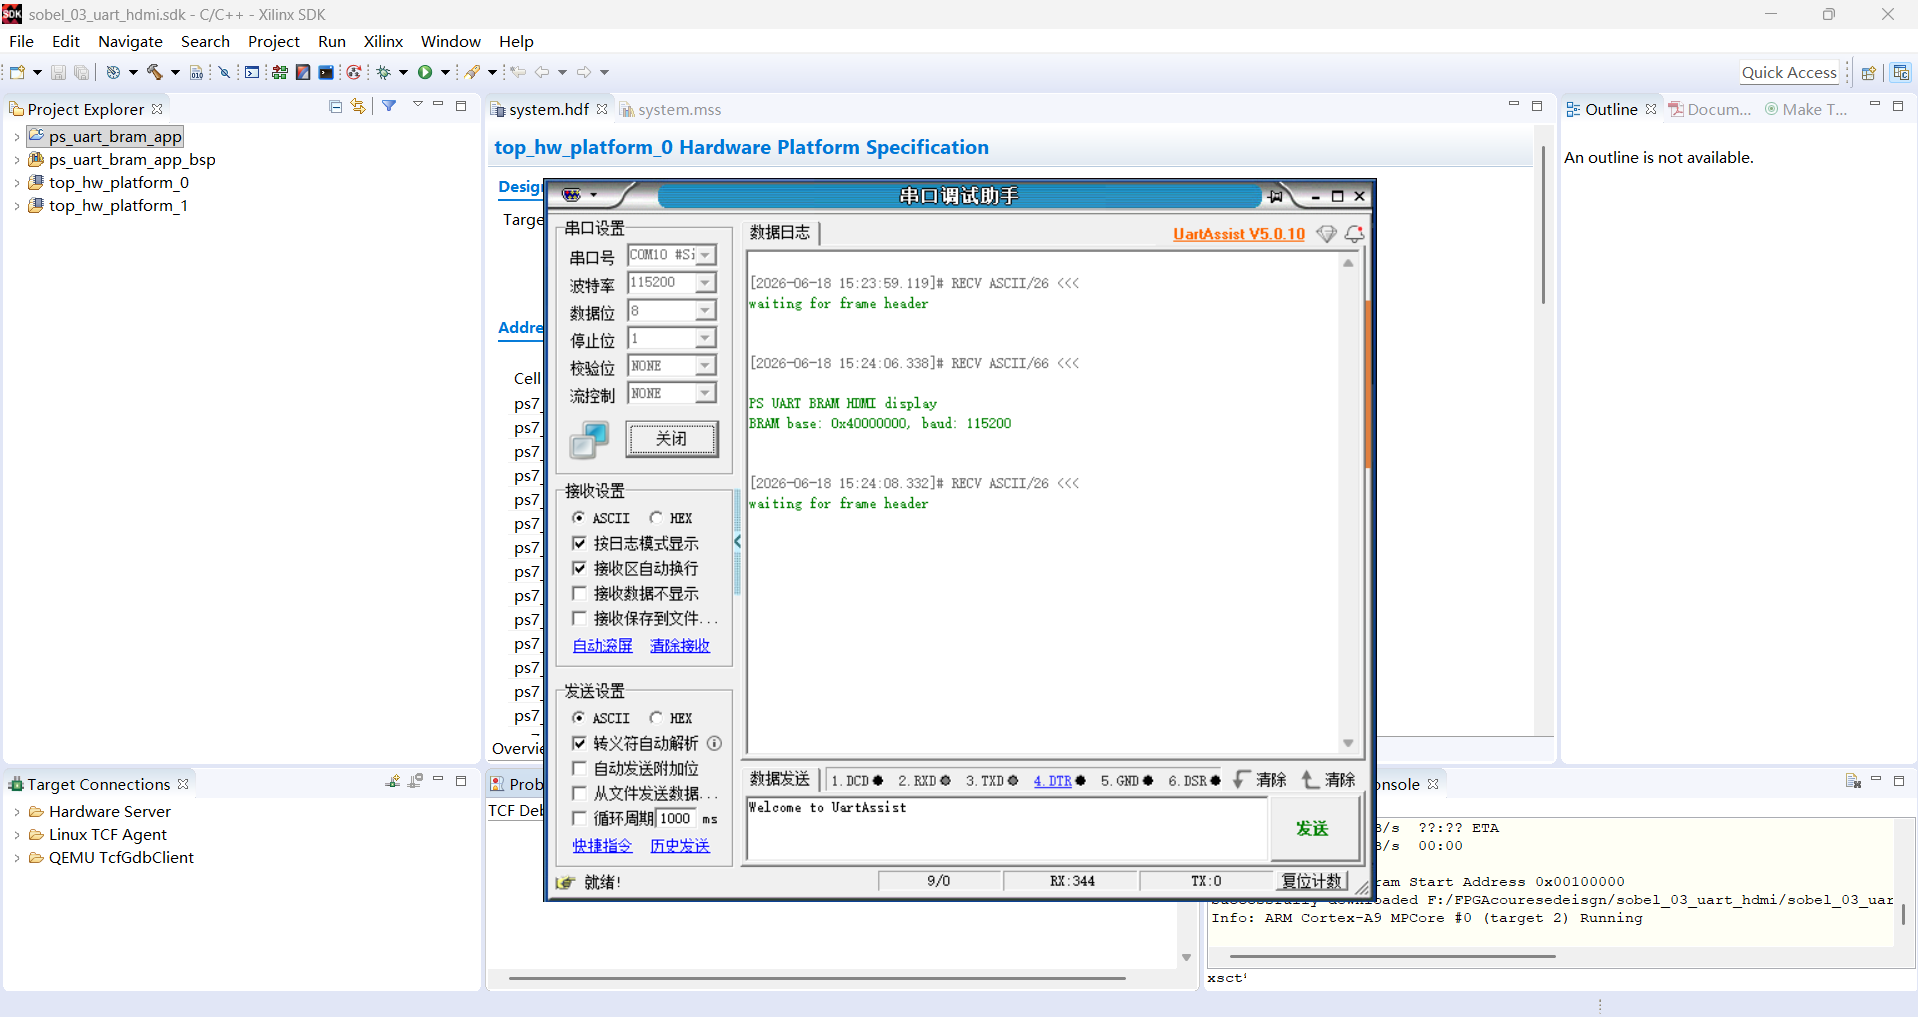
\includegraphics[width=0.32\textwidth]{exp3_serial.png}}
\caption{实验3资源、时序与串口验证}
\label{fig:exp3-timing}
\end{figure}

该实验的调试重点在串口占用和帧格式一致性。上位机发送时串口会被占用，不能同时用串口助手打开同一个 COM 口；需要在上位机停止或关闭后，再用串口助手查看 PS 端打印信息。

\section{实验4：UART Sobel 图像处理与 HDMI 显示}

\subsection{基础功能}

实验 4 把实验 3 的 UART 图像输入和实验 2 的 Sobel 处理组合起来。PC 端发送图片或摄像头画面，PS 写入 BRAM，PL 端读取后进行灰度和 Sobel 计算，最后 HDMI 显示边缘结果。

\figtwocol{exp4_camera.jpg}{摄像头输入边缘显示}{exp4_image.jpg}{图片输入边缘显示}{实验4基础功能现象}{fig:exp4-basic}

两种输入来源都能显示出明显边缘，说明 UART 输入、BRAM 缓存、Sobel 核心和 HDMI 输出之间能够连续工作。

\subsection{扩展实现}

扩展功能仍然采用反色显示思路，但这一次反色作用在 UART 输入图像的 Sobel 结果上。由于输入图像来自 PC 端，实际效果比固定图案更能体现边缘检测在不同图片上的变化。

\figone{0.62}{exp4_extend.jpg}{实验4 Sobel 反色扩展显示}{fig:exp4-extend}

\subsection{资源、时序与串口验证}

\begin{figure}[H]
\centering
\subfigure[资源占用]{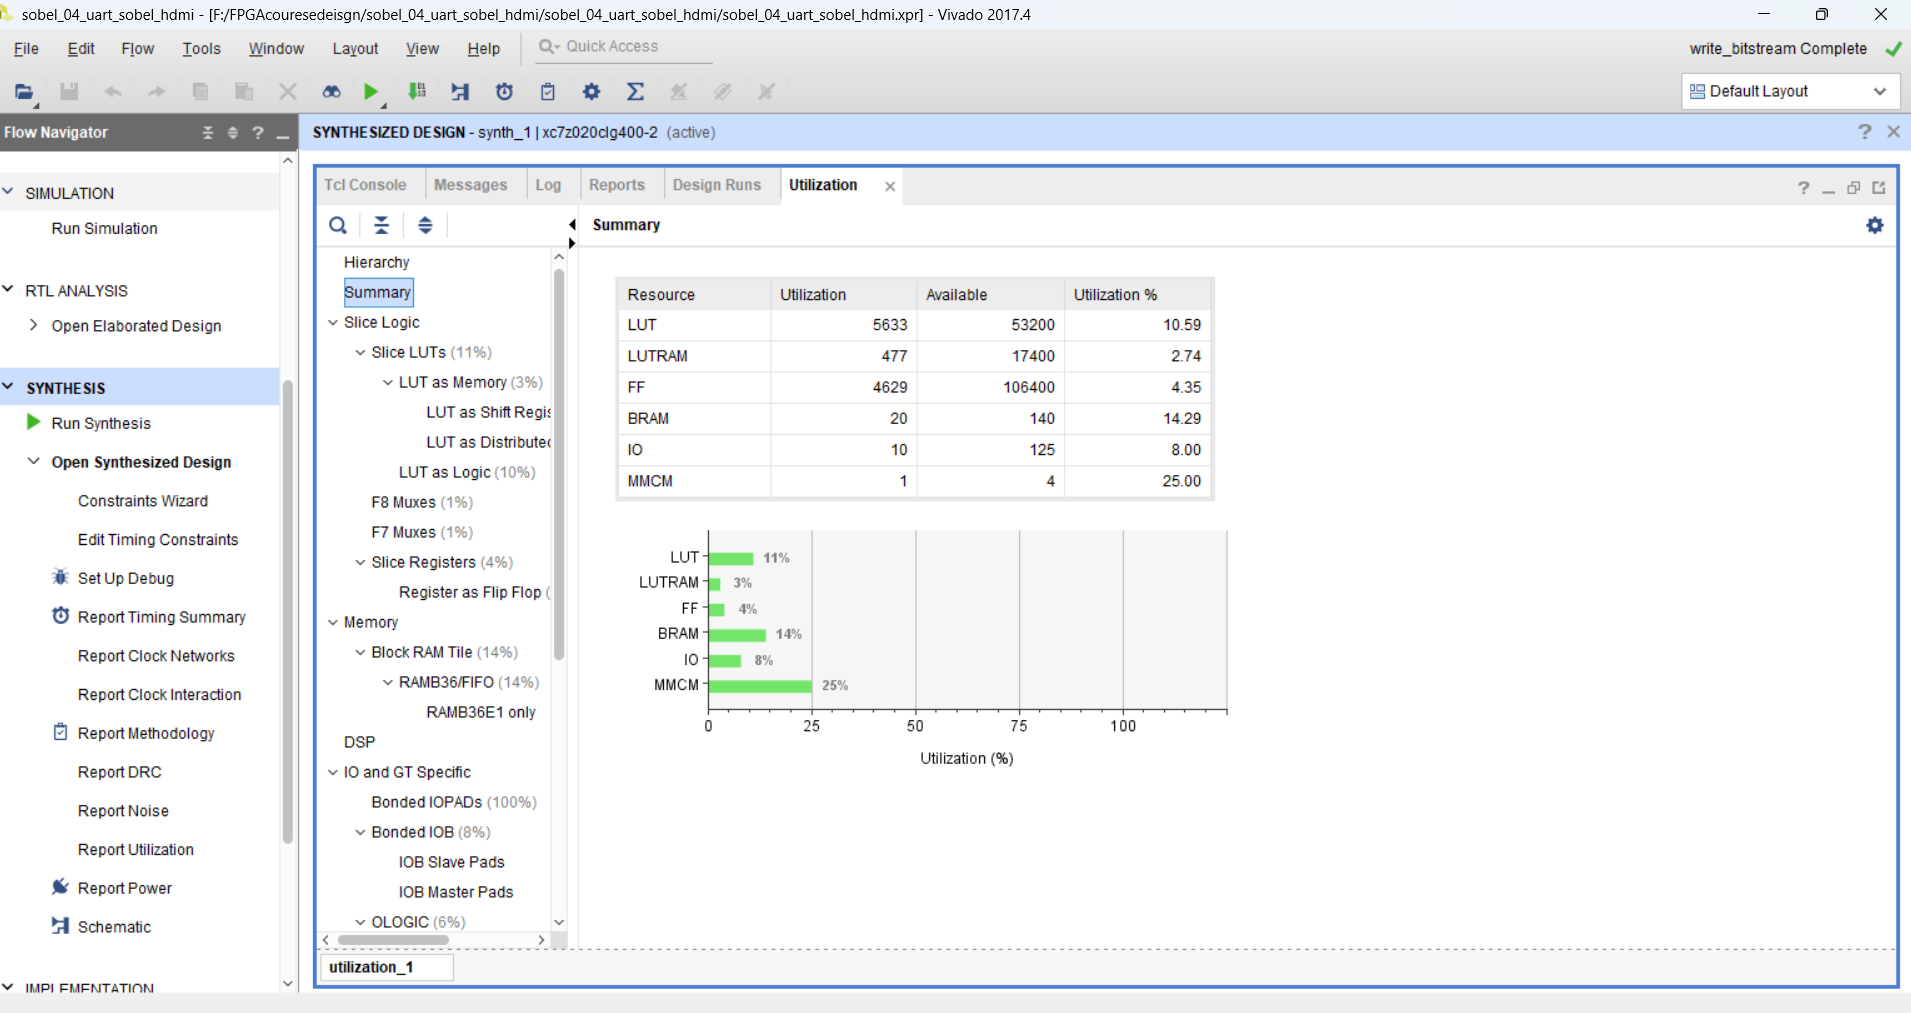
\includegraphics[width=0.32\textwidth]{exp4_utilization.png}}
\subfigure[时序结果]{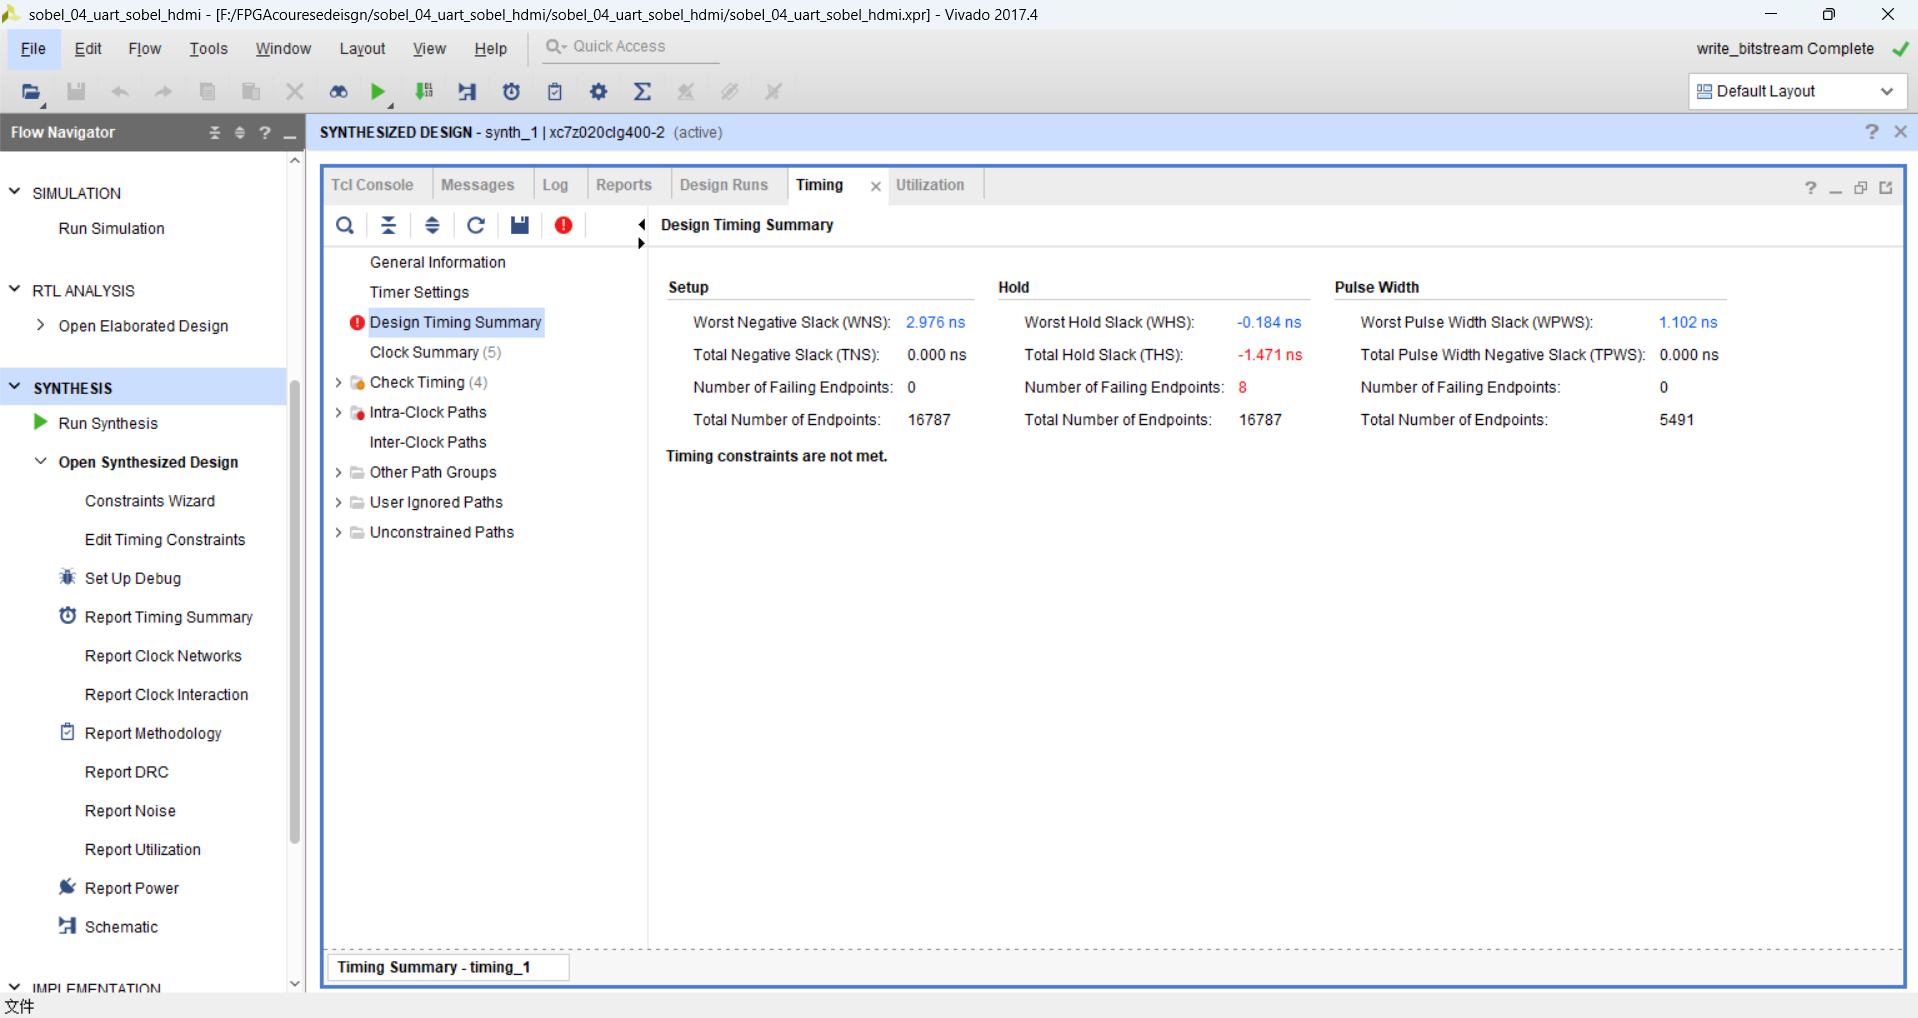
\includegraphics[width=0.32\textwidth]{exp4_timing.png}}
\subfigure[串口信息]{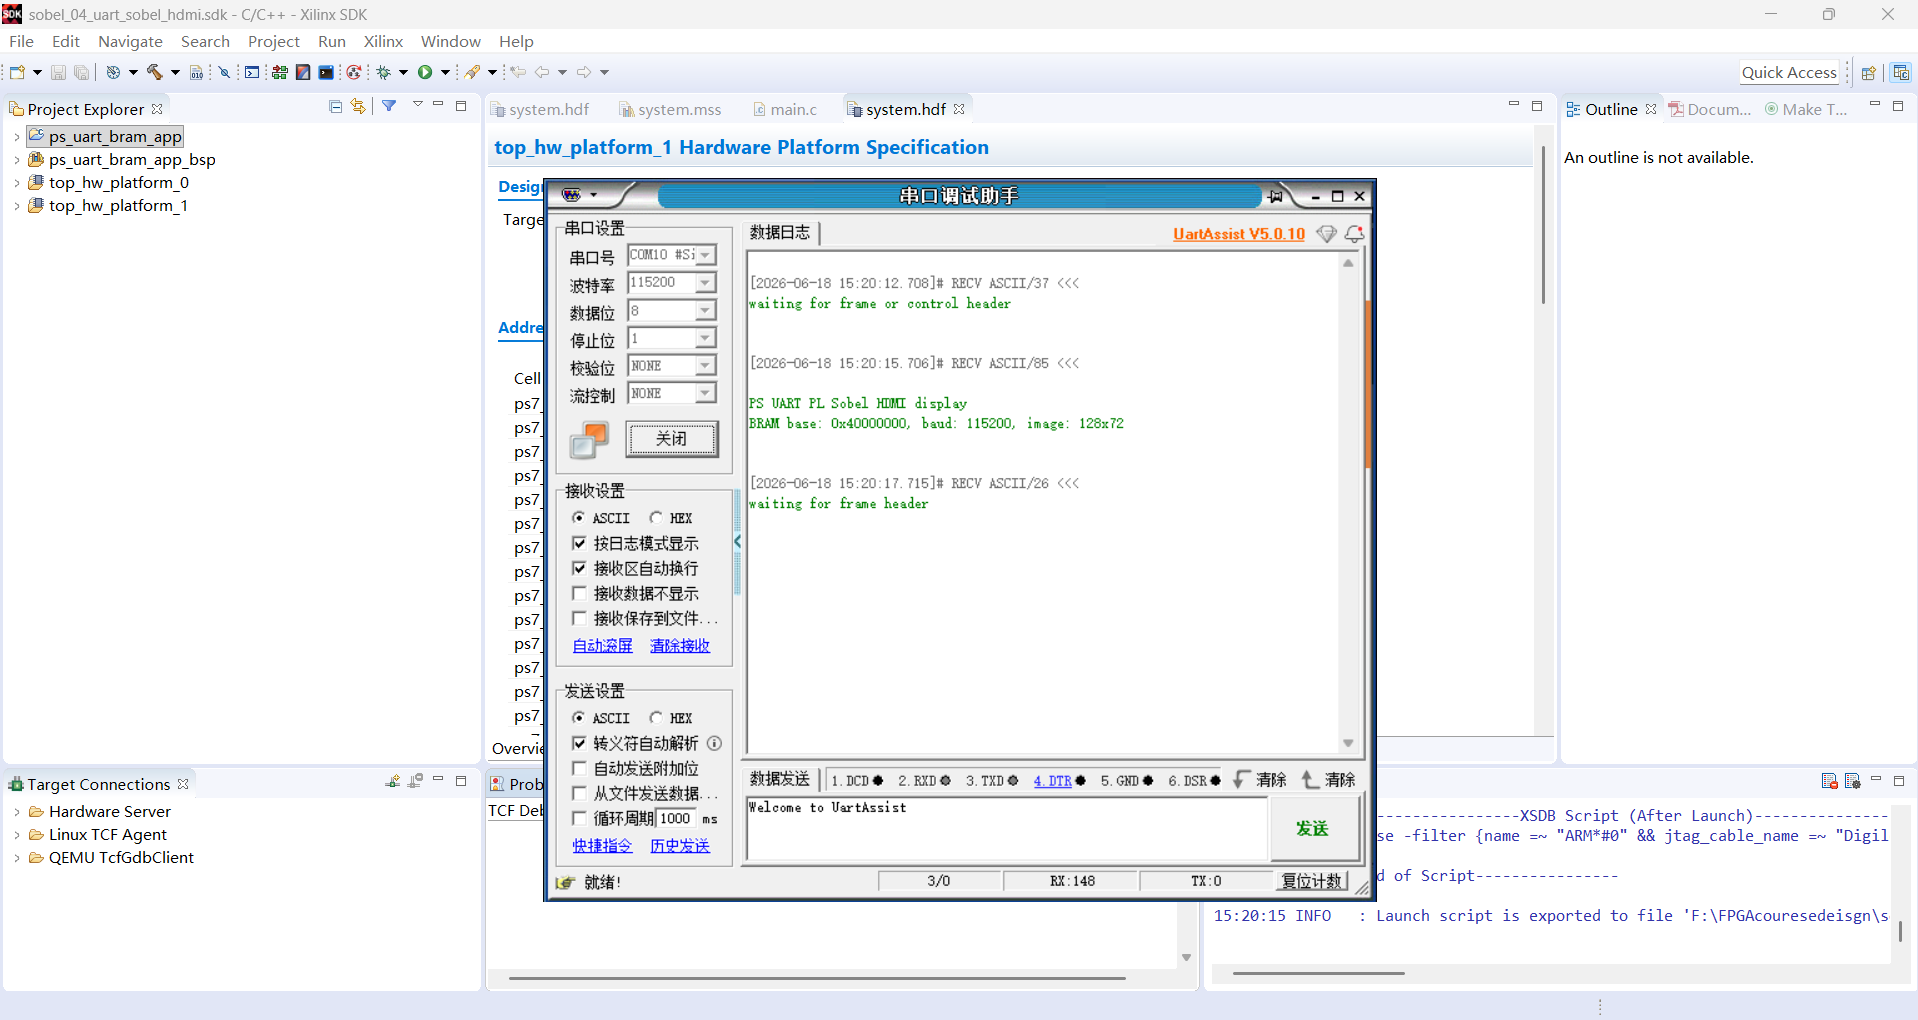
\includegraphics[width=0.32\textwidth]{exp4_serial.png}}
\caption{实验4资源、时序与串口验证}
\label{fig:exp4-timing}
\end{figure}

实验 4 的现象说明，在真实输入图像下，边缘检测结果仍能保持稳定输出。资源占用相比实验 3 增加，主要来自灰度转换、行缓存和 Sobel 计算逻辑。

\section{实验5：PC 控制显示与综合拓展}

\subsection{基础功能}

实验 5 在实验 4 的基础上加入显示控制。上位机不仅发送图像，还能发送控制命令，让 FPGA 端切换原图、灰度、边缘、叠加等显示模式，并调整 Sobel 阈值。PS 端通过控制帧解析命令，将模式、阈值和叠加开关写入 BRAM 后部的控制地址；PL 端显示模块读取这些控制字，改变输出画面。

\begin{lstlisting}[language=C,caption={实验5 PS 端控制地址定义}]
#define CTRL_MODE_ADDR      (FRAMEBUFFER_BASEADDR + 0x9000U)
#define CTRL_THRESHOLD_ADDR (FRAMEBUFFER_BASEADDR + 0x9004U)
#define CTRL_OVERLAY_ADDR   (FRAMEBUFFER_BASEADDR + 0x9008U)
\end{lstlisting}

控制帧采用 \verb|A5 5A cmd value| 形式，其中 \verb|cmd=1| 表示显示模式，\verb|cmd=2| 表示阈值，\verb|cmd=3| 表示叠加开关。这样做的好处是图像数据帧和控制命令帧可以共用同一个 UART 通道，但解析状态机可以通过不同帧头区分。

\begin{figure}[H]
\centering
\subfigure[上位机与串口控制]{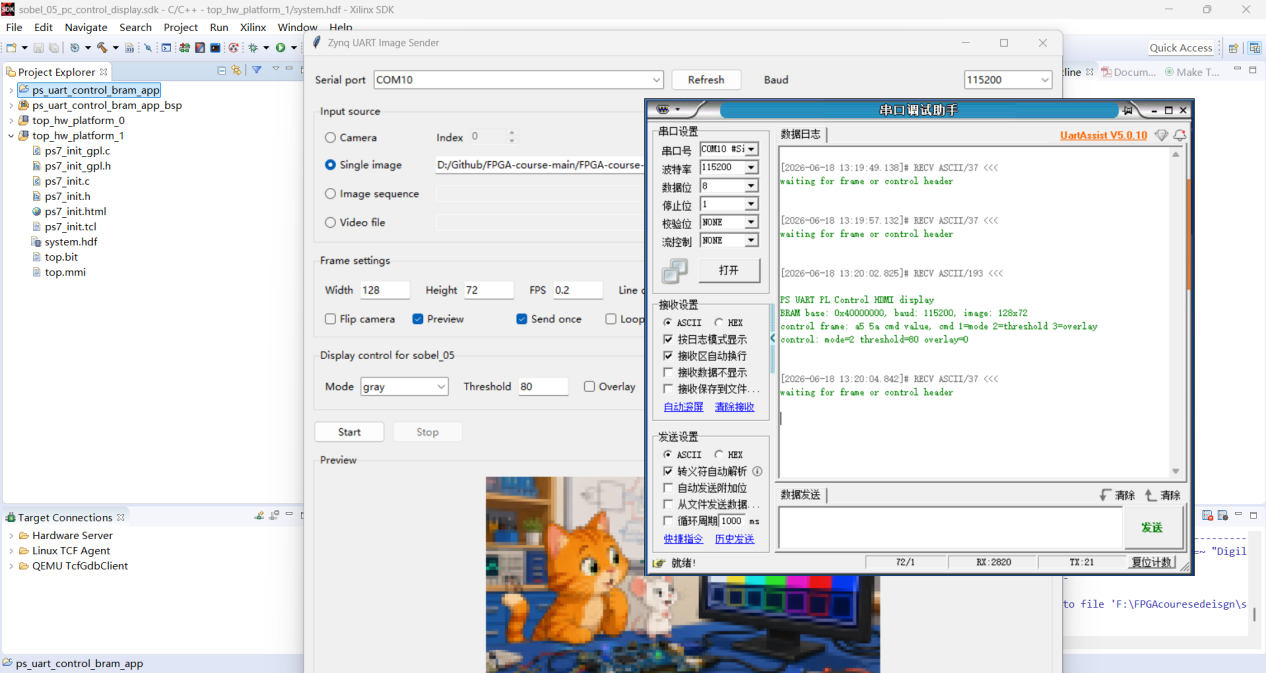
\includegraphics[width=0.46\textwidth]{exp5_basic_docx/exp5_basic_docx_04.png}}
\subfigure[摄像头/图片显示]{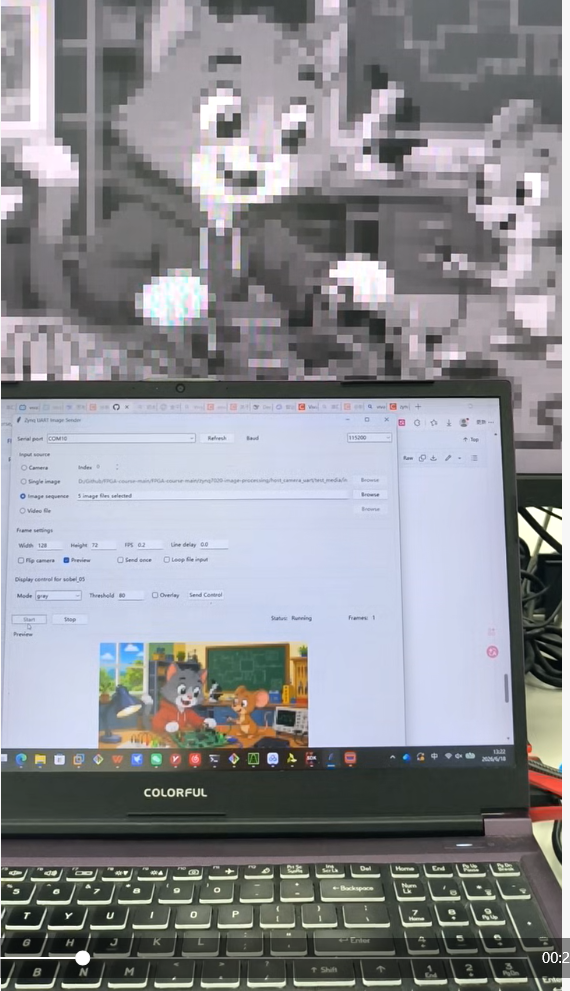
\includegraphics[width=0.46\textwidth]{exp5_basic_docx/exp5_basic_docx_05.png}}
\caption{实验5基础功能联调记录}
\label{fig:exp5-basic-gui}
\end{figure}

\begin{figure}[H]
\centering
\subfigure[灰度显示]{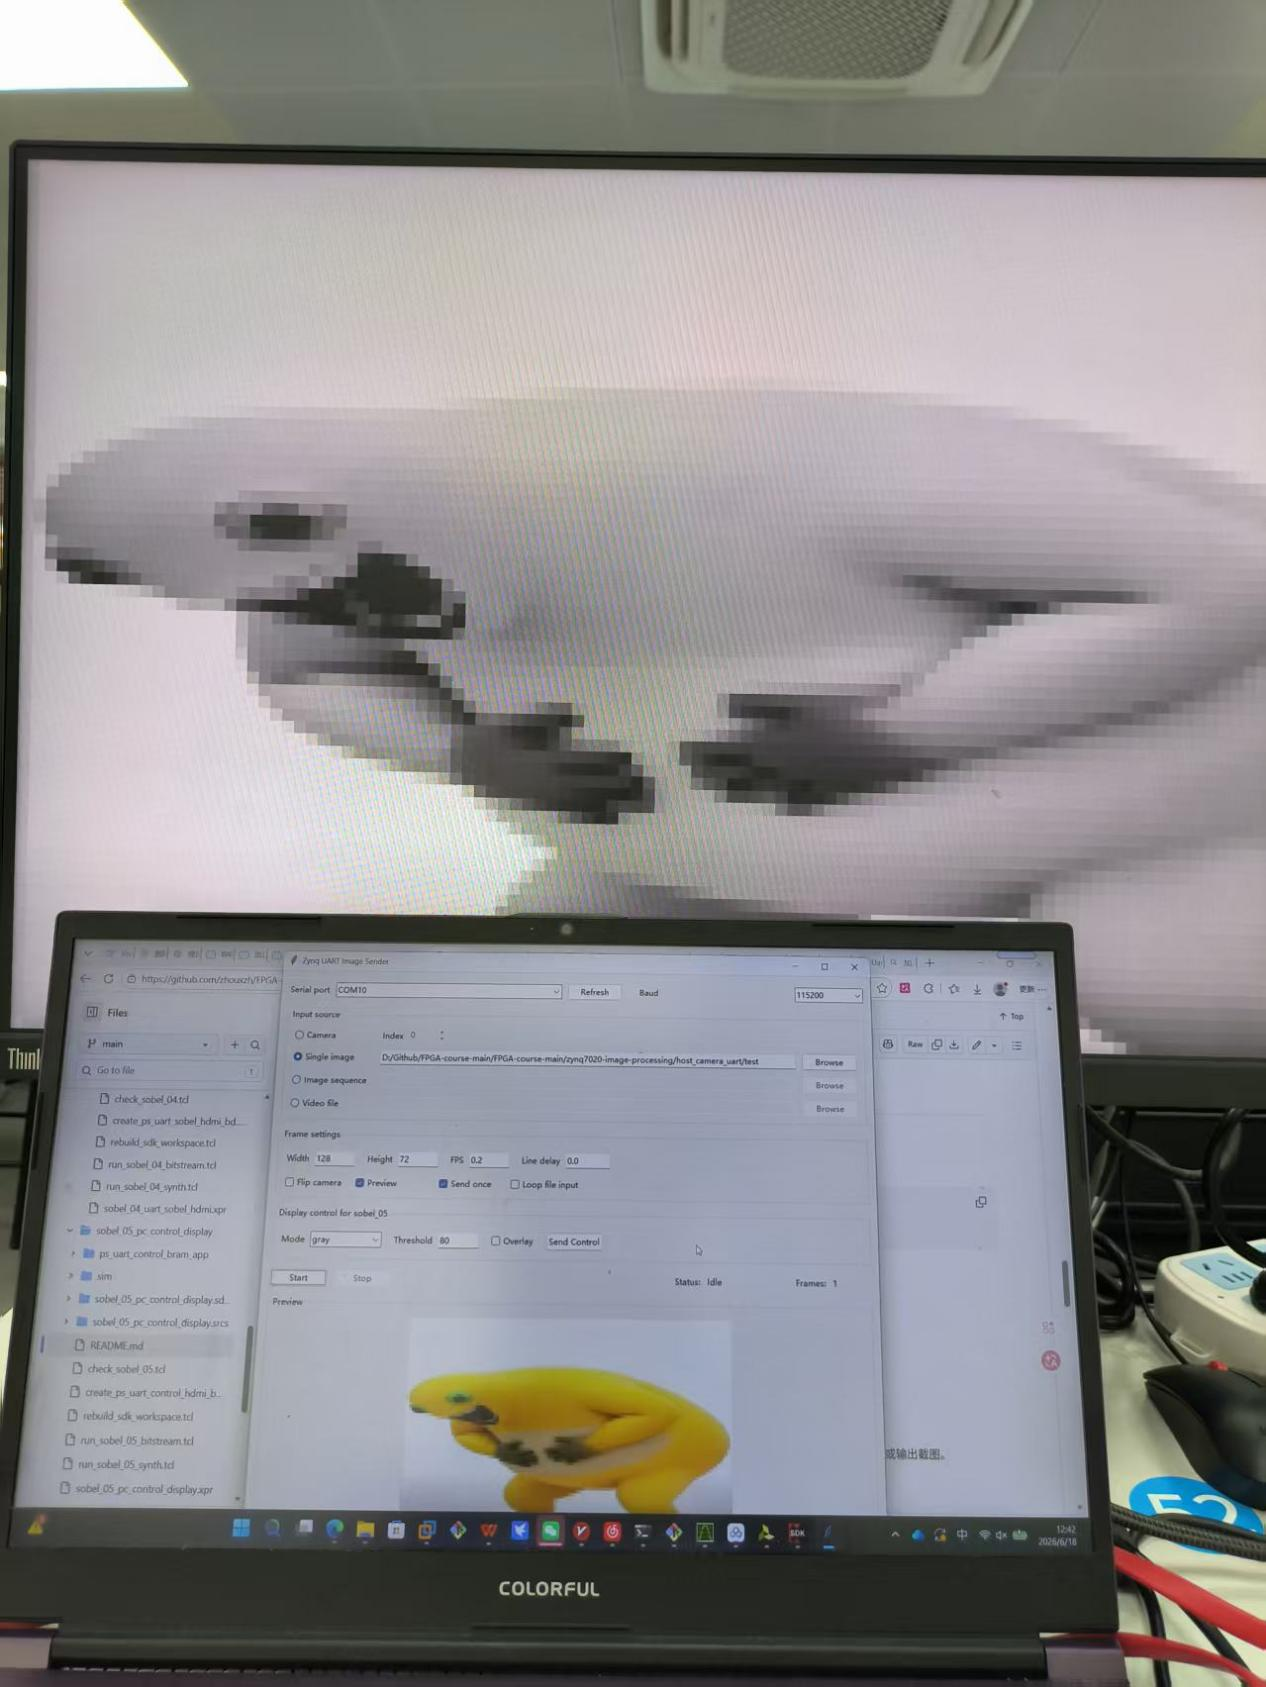
\includegraphics[width=0.30\textwidth]{exp5_basic_docx/exp5_basic_docx_10.jpeg}}
\subfigure[边缘显示]{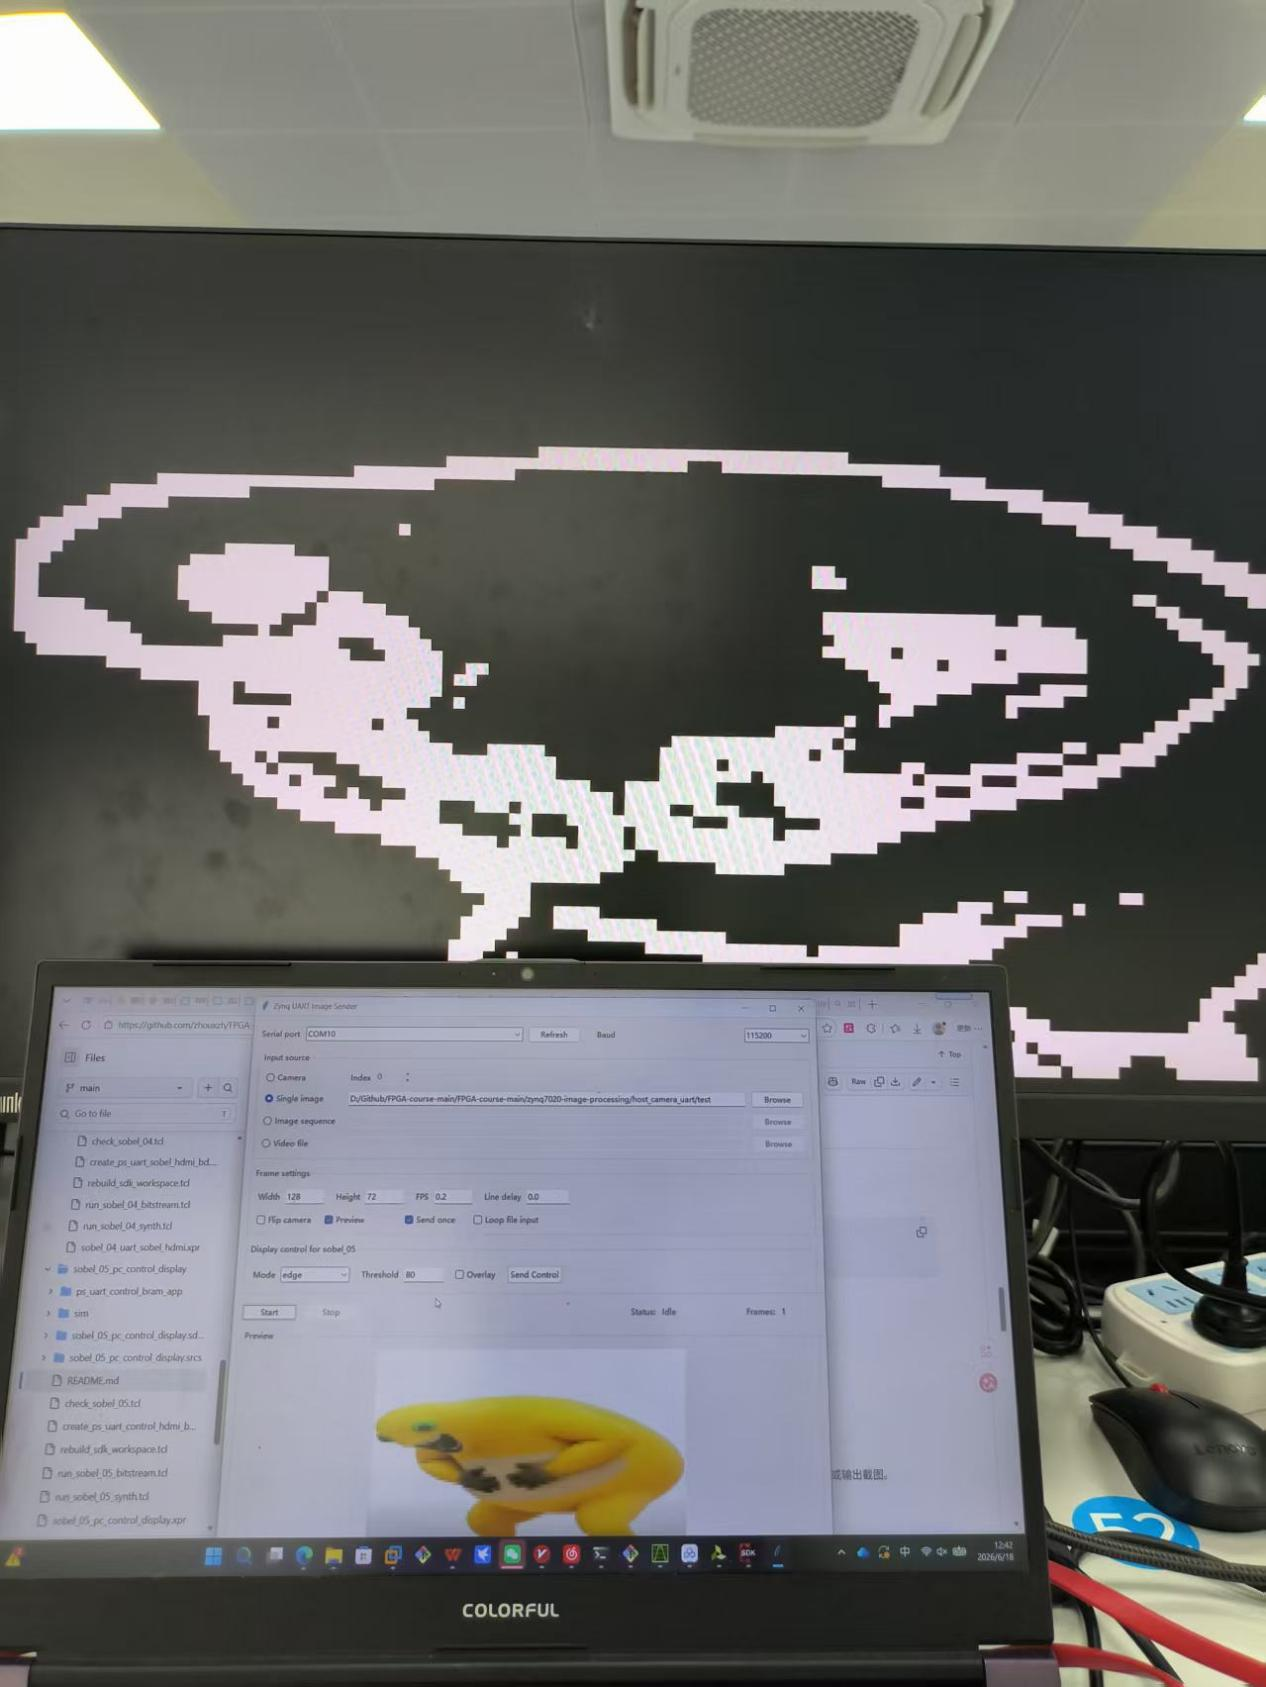
\includegraphics[width=0.30\textwidth]{exp5_basic_docx/exp5_basic_docx_11.jpeg}}
\subfigure[叠加显示]{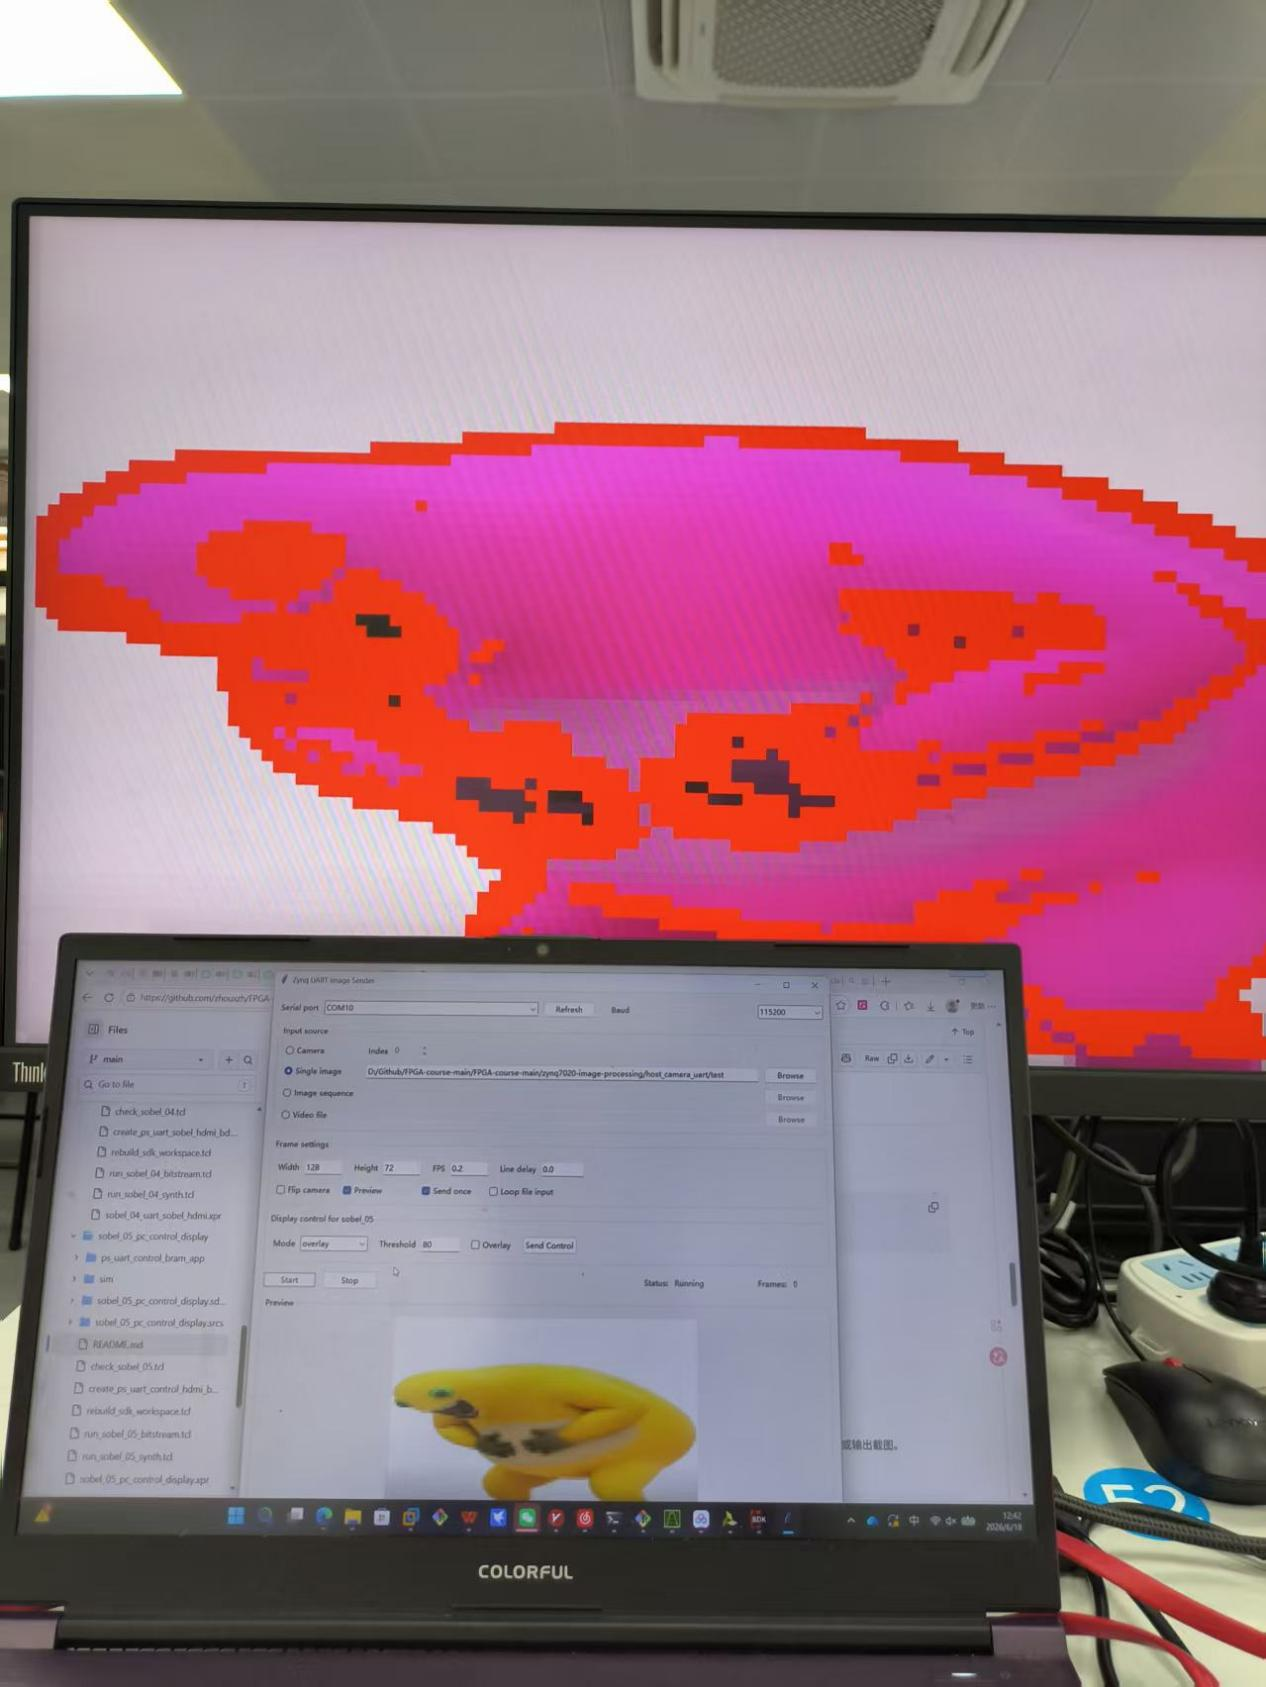
\includegraphics[width=0.30\textwidth]{exp5_basic_docx/exp5_basic_docx_12.jpeg}}
\caption{实验5不同显示模式现象}
\label{fig:exp5-basic-modes}
\end{figure}

在基础功能验证中，原图、灰度、边缘和叠加模式都能通过上位机切换；阈值改变后，边缘提取的粗细和保留程度也会变化。这个实验把前面几次单独验证过的 UART、BRAM、Sobel 和 HDMI 显示串成了可交互系统。

\subsection{综合拓展目标}

综合拓展选择“基于 \verb|sobel_05| 的上位机与输入规格扩展”。本组实际完成的重点是上位机侧输入规格改造：在原来固定 \verb|128 x 72| 的基础上，加入目标尺寸选择、缩放策略选择和新增图片输入规格验证，同时保持实验 5 原有显示控制命令可用。

这里需要说明一点：最终上板验证仍以原硬件链路的 \verb|128 x 72| 为主，新增尺寸和缩放策略主要在上位机预处理与发送链路中完成验证。也就是说，扩展的主思路是“上位机统一预处理后再送入 FPGA”，而不是完全重写 PL 端 HDMI 放大和 BRAM 地址计算。这样可以在不大幅增加硬件改动风险的前提下，完成输入来源与输入规格的扩展验证。

\subsection{上位机输入规格扩展}

上位机改动集中在 \verb|camera_uart_sender.py| 和 \verb|camera_uart_gui.py|。命令行版本加入尺寸预设和缩放模式，GUI 版本加入 Size preset、Width、Height、Fit 等控件。新增的尺寸预设如下：

\begin{lstlisting}[language=Python,caption={上位机尺寸预设}]
SIZE_PRESETS = {
    "128x72":  (128, 72),
    "128x80":  (128, 80),
}
\end{lstlisting}

缩放策略分为三种：

\begin{itemize}
    \item \verb|fit|：保持比例缩放，空白处用黑边填充；
    \item \verb|stretch|：直接拉伸到目标尺寸，画面可能变形；
    \item \verb|crop|：保持比例并居中裁剪，画面填满目标区域。
\end{itemize}

\begin{figure}[H]
\centering
\subfigure[128x80 stretch]{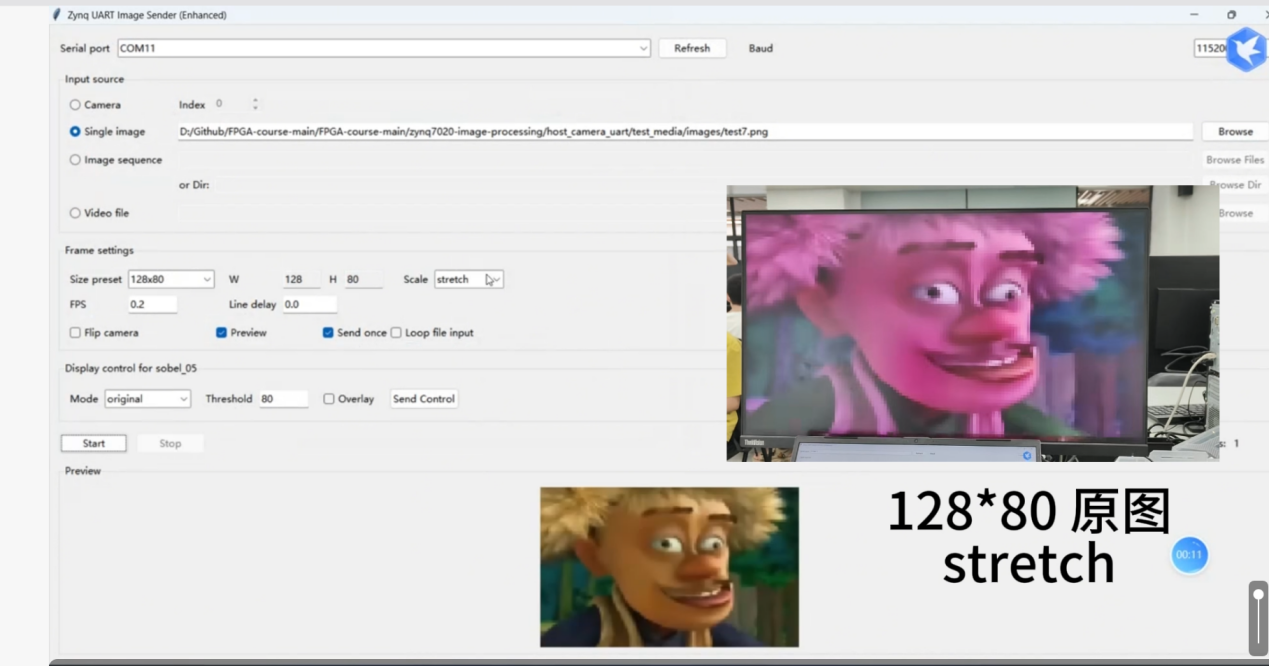
\includegraphics[width=0.46\textwidth]{exp5_extend_docx/exp5_extend_docx_03.png}}
\subfigure[128x80 crop]{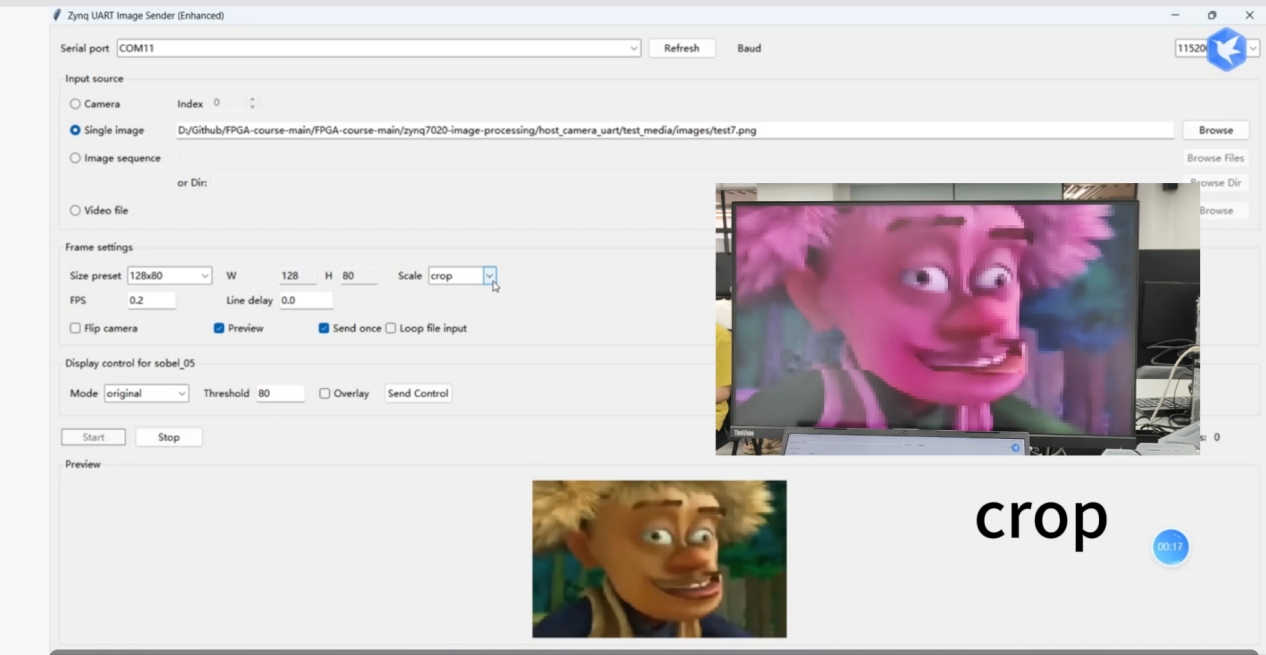
\includegraphics[width=0.46\textwidth]{exp5_extend_docx/exp5_extend_docx_04.png}}
\caption{实验5拓展：新增输入规格与缩放策略}
\label{fig:exp5-extend-size}
\end{figure}

从图 \ref{fig:exp5-extend-size} 可以看到，同一张原始图片在不同缩放策略下会进入不同的预处理结果。对于 FPGA 端而言，接收的仍是连续 RGB888 像素流；差异主要体现在上位机送出的像素内容。

\subsection{显示控制保持兼容}

综合拓展没有去掉实验 5 的显示控制。GUI 中仍然可以选择 \verb|original|、\verb|gray|、\verb|edge|、\verb|overlay|，并设置阈值。上位机发送图像前或发送过程中都可以排队控制命令，PS 端收到后更新控制字。

\begin{figure}[H]
\centering
\subfigure[灰度模式]{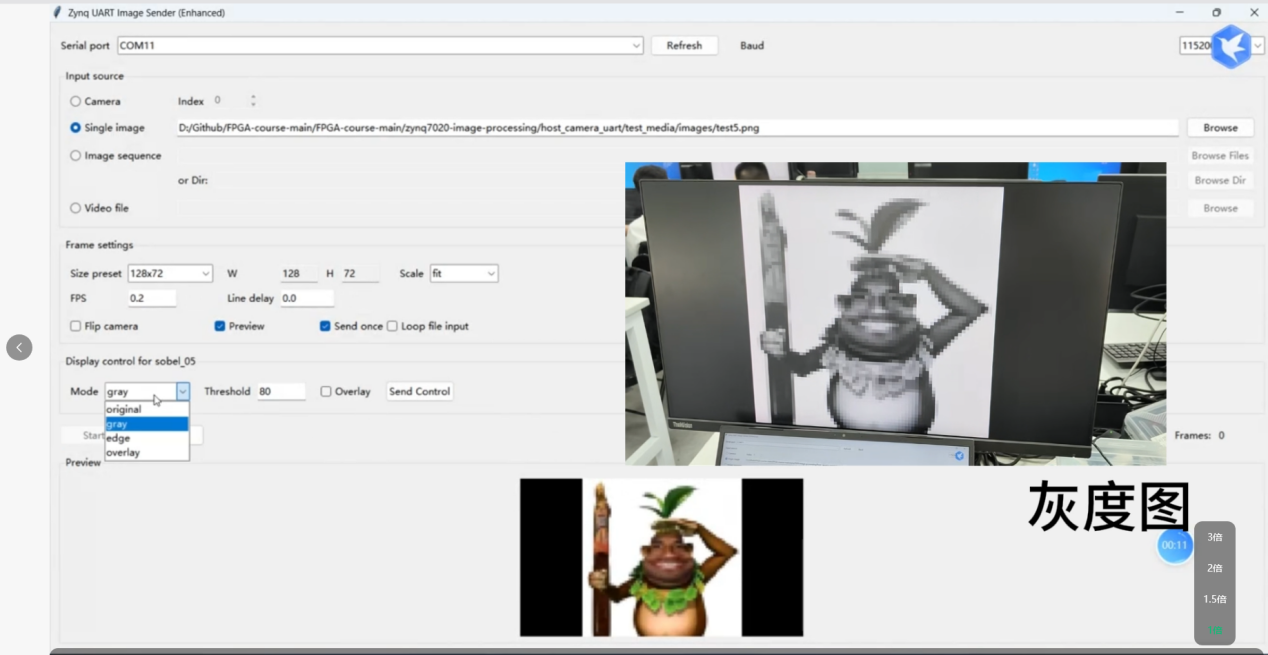
\includegraphics[width=0.30\textwidth]{exp5_extend_docx/exp5_extend_docx_16.png}}
\subfigure[边缘模式]{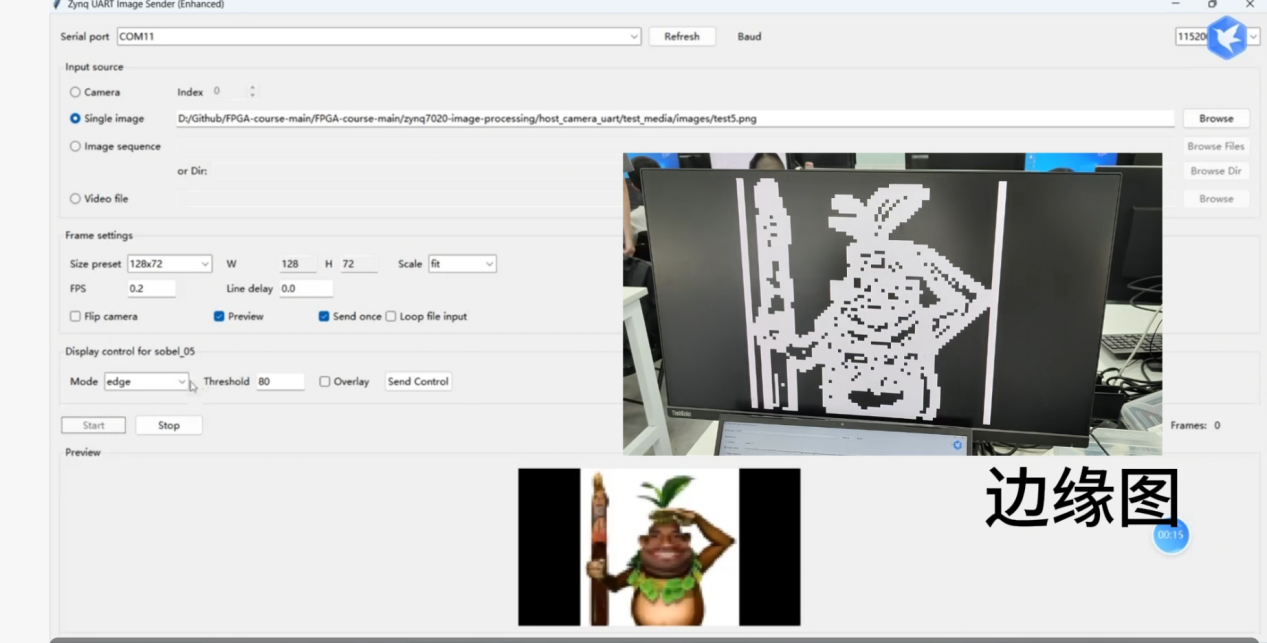
\includegraphics[width=0.30\textwidth]{exp5_extend_docx/exp5_extend_docx_17.png}}
\subfigure[叠加模式]{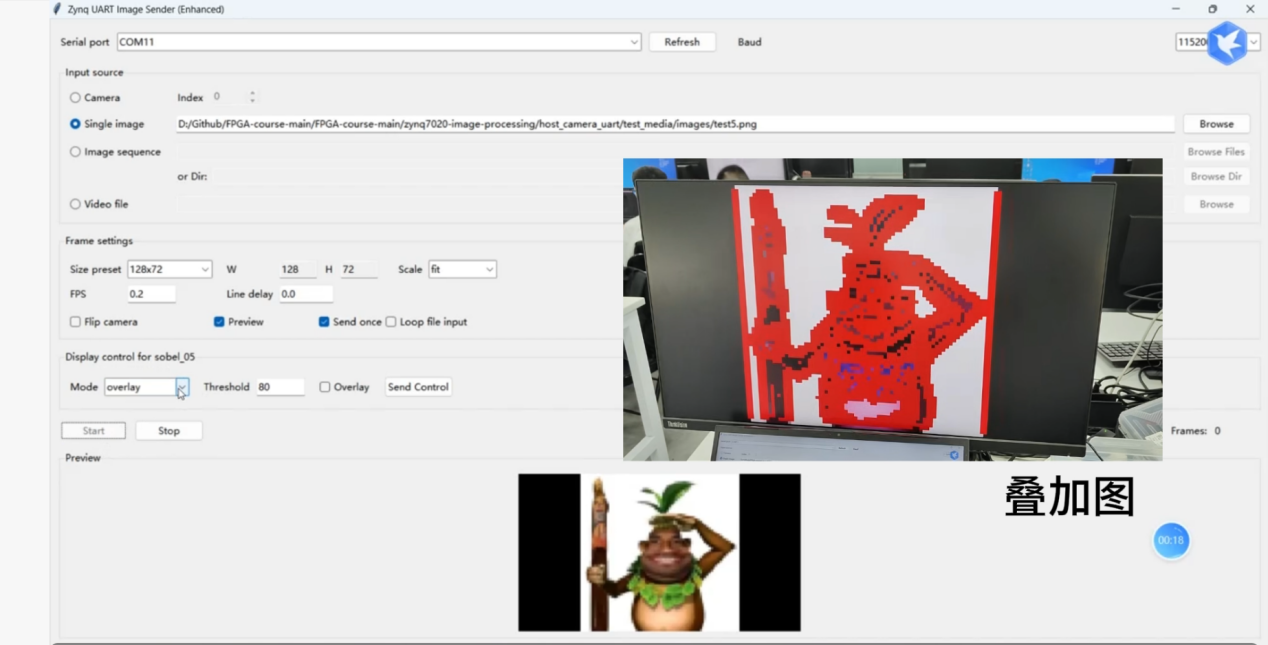
\includegraphics[width=0.30\textwidth]{exp5_extend_docx/exp5_extend_docx_18.png}}
\caption{实验5拓展后显示控制仍可使用}
\label{fig:exp5-extend-control}
\end{figure}

阈值控制也保留了下来。阈值越低，更多弱边缘会被保留；阈值越高，只保留强边缘。这个现象在演示中通过多组阈值切换完成验证。

\subsection{实验五资源与时序}

\figtwocol{exp5_utilization.png}{综合拓展资源占用}{exp5_timing.png}{综合拓展时序摘要}{实验5综合拓展综合实现结果}{fig:exp5-resource}

从资源占用看，综合拓展仍然主要消耗 LUT、FF 和 BRAM。BRAM 用于图像缓存，逻辑资源用于 HDMI 时序、灰度/Sobel 流水线和控制选择。时序报告中 Setup、Hold 和 Pulse Width 是主要关注项；在实际演示中，系统能够完成 bitstream 生成、SDK 下载和上板显示，说明设计在当前实验频率下可以运行。

\section{调试问题与处理}

\subsection{串口占用问题}

UART 实验中最容易遇到的问题是串口被多个程序同时打开。例如上位机正在向 COM 口发送图像时，串口助手无法同时打开该端口；反过来，如果串口助手占用了端口，上位机也会发送失败。处理方法是一次只保留一个串口程序连接，观察调试信息时先停止上位机发送。

\subsection{图像尺寸与帧格式问题}

基础工程对图像尺寸要求严格，PS 端会检查宽度、高度和 RGB888 格式。如果上位机发送的帧头尺寸和工程定义不一致，PS 会拒绝接收或等待下一帧。综合拓展中因此采用上位机预处理策略：先在 PC 端统一缩放或裁剪，再按工程当前支持的帧格式发送。

\subsection{HDMI 画面调试}

HDMI 显示问题通常不容易只看代码判断，需要结合显示器现象、串口信息和 Vivado 资源/时序报告一起看。比如画面错位时，需要检查坐标映射和 BRAM 地址；图像不刷新时，需要检查 UART 帧是否完整；显示模式不切换时，需要检查控制字地址是否和 PL 端读取地址一致。

\subsection{报告与仓库整理}

课程提交要求包含工程文件和 Markdown 报告。前期图片路径如果直接引用本地绝对路径，在 GitHub 页面上无法显示；后续统一把报告图片放入对应工程的 \verb|picture| 或 \verb|build| 目录，并使用相对路径引用。综合报告则把图片统一复制到 \verb|figures|，便于 LaTeX 编译和仓库保存。

\section{总结}

这次课程设计从一个纯 RTL Sobel 仿真开始，最后做到 PC 上位机、PS 程序、PL 图像流水线和 HDMI 输出联动，过程里最明显的感受是：FPGA 实验不只是把某一个模块写对，还要让数据格式、地址、时序和外设行为全部对齐。很多问题单看一个模块都像是对的，真正上板之后才会暴露在串口、显示器和波形里。

基础实验 0 到 5 分别验证了仿真、HDMI、Sobel、UART、PS/PL 联调和显示控制。小扩展让我们在原工程上做了可见、可验证的修改，例如红色边框、反色边缘和 UART 图像边框。综合拓展则把工作重心放在上位机输入规格上，通过尺寸预设和缩放策略，让输入图像进入 FPGA 前更加可控，同时保留原有显示控制链路。

从小组协作看，PL 端、PS 端、上位机和验证材料相互依赖很强。单独完成某一段并不难，难的是让每一段的约定一致。经过这次实验，我们对 ZYNQ 平台中 PS 与 PL 的分工、BRAM 作为图像缓存的作用、UART 帧协议设计以及 HDMI 显示调试都有了更具体的认识。

\appendix

\section{主要提交目录}

\begin{itemize}
    \item \verb|sobel_00_rtl_sim|：Sobel RTL 仿真工程与仿真报告。
    \item \verb|sobel_01_hdmi_pattern_expand|：实验 1 扩展工程与实验报告。
    \item \verb|sobel_02_hdmi_sobel_expand|：实验 2 扩展工程与实验报告。
    \item \verb|sobel_03_uart_hdmi_expand|：实验 3 扩展工程与实验报告。
    \item \verb|sobel_04_uart_sobel_hdmi_expand|：实验 4 扩展工程与实验报告。
    \item \verb|sobel_05_pc_control_display_expand|：实验 5 基础与综合拓展工程。
    \item \verb|host_camera_uart_enhanced|：综合拓展上位机程序。
    \item \verb|报告|：各实验 Markdown 报告、扩展说明和本综合报告。
\end{itemize}

\section{参考资料}

\begin{thebibliography}{99}
\bibitem{course} 周贤中. FPGA-course/zynq7020-image-processing 课程实验仓库.
\bibitem{xilinx} AMD Xilinx. Vivado Design Suite User Guide.
\bibitem{verilog} 夏宇闻. Verilog 数字系统设计教程. 北京航空航天大学出版社.
\end{thebibliography}

\end{document}
